\documentclass[11pt,a4paper]{article}

% Importar preámbulo con paquetes
%%%%%%%%%%%%%%%%%%%%%%%%%%%%%%%%%%%%%%%%%
% Wenneker Assignment
% Structure Specification File
% Version 2.0 (12/1/2019)
%
% This template originates from:
% http://www.LaTeXTemplates.com
%
% Authors:
% Vel (vel@LaTeXTemplates.com)
% Frits Wenneker
%
% License:
% CC BY-NC-SA 3.0 (http://creativecommons.org/licenses/by-nc-sa/3.0/)
% 
%%%%%%%%%%%%%%%%%%%%%%%%%%%%%%%%%%%%%%%%%

%----------------------------------------------------------------------------------------
%	PACKAGES AND OTHER DOCUMENT CONFIGURATIONS
%----------------------------------------------------------------------------------------
\usepackage[spanish]{babel} %idioma español
\addto\captionsspanish{\renewcommand{\tablename}{Tabla}} % Para que las tablas no se llamen Cuadros
\usepackage[utf8]{inputenc} %tildes en español

\usepackage[shortlabels]{enumitem}
\usepackage[backend=biber,style=numeric]{biblatex}
\usepackage[shortlabels]{enumitem}
\addbibresource{referencias.bib} %Import the bibliography file
\usepackage{lipsum}% http://ctan.org/pkg/lipsum
\usepackage{subcaption}
\captionsetup{compatibility=false}
\usepackage{float}
\usepackage[makeroom]{cancel}
\usepackage{siunitx}
\usepackage[table,xcdraw]{xcolor}
\usepackage{tabularx}
\usepackage{array}
\usepackage{pdflscape}


%nuevos---------------
\usepackage{graphicx}
\usepackage{changepage}
\renewcommand{\labelenumi}{\theenumi.}
\usepackage{amssymb}
\usepackage{caption}
\usepackage{chngcntr} %para poder poner que se enumeren las cosas de formas distintas.
\usepackage{multirow}
\usepackage[skip=4pt plus1pt, indent=10pt]{parskip}
\usepackage{color}
\usepackage{tabularx} % 
\usepackage{cite}






\usepackage{hyperref} %índice clickable
\hypersetup{
    colorlinks,
    citecolor=black,
    filecolor=black,
    linkcolor=black,
    urlcolor=black
}


\usepackage[mathscr]{euscript}

% Copied from mathrsfs.sty
\DeclareSymbolFont{rsfs}{U}{rsfs}{m}{n}
\DeclareSymbolFontAlphabet{\mathscrsfs}{rsfs}


\usepackage{amsmath, amsfonts, amsthm} % Math packages

\usepackage{listings}
\usepackage{xcolor}
\usepackage{pdfpages}

\lstdefinelanguage{FreeFem++}{
    alsodigit = {-},
    keywords = {problem, int2d, on}
}

\definecolor{codegreen}{rgb}{0,0.6,0}
\definecolor{codegray}{rgb}{0.5,0.5,0.5}
\definecolor{codepurple}{rgb}{0.58,0,0.82}
\definecolor{backcolour}{rgb}{0.95,0.95,0.92}

\lstdefinestyle{mystyle}{
    backgroundcolor=\color{backcolour},   
    commentstyle=\color{codegreen},
    keywordstyle=\color{magenta},
    numberstyle=\tiny\color{codegray},
    stringstyle=\color{codepurple},
    basicstyle=\ttfamily\footnotesize,
    breakatwhitespace=false,         
    breaklines=true,                 
    captionpos=b,                    
    keepspaces=true,                 
    numbers=left,                    
    numbersep=5pt,                  
    showspaces=false,                
    showstringspaces=false,
    showtabs=false,                  
    tabsize=2
}


% \usepackage[english]{babel} % English language hyphenation

\usepackage{graphicx} % Required for inserting images
\graphicspath{{Figures/}{./}} % Specifies where to look for included images (trailing slash required)

\usepackage{booktabs} % Required for better horizontal rules in tables

\numberwithin{equation}{section} % Number equations within sections (i.e. 1.1, 1.2, 2.1, 2.2 instead of 1, 2, 3, 4)
\numberwithin{figure}{section} % Number figures within sections (i.e. 1.1, 1.2, 2.1, 2.2 instead of 1, 2, 3, 4)
\numberwithin{table}{section} % Number tables within sections (i.e. 1.1, 1.2, 2.1, 2.2 instead of 1, 2, 3, 4)

\setlength\parindent{0pt} % Removes all indentation from paragraphs

\usepackage{enumitem} % Required for list customisation
\setlist{noitemsep} % No spacing between list items

%Maider
\usepackage{longtable} % Para tablas que abarcan varias páginas
\usepackage{lscape} % Para rotar la tabla en página horizontal
\usepackage{tikz}
\usetikzlibrary{shapes.geometric, arrows}

%----------------------------------------------------------------------------------------
%	DOCUMENT MARGINS
%----------------------------------------------------------------------------------------

\usepackage{geometry} % Required for adjusting page dimensions and margins

\geometry{
	paper=a4paper, % Paper size, change to letterpaper for US letter size
	top=2.5cm, % Top margin
	bottom=3cm, % Bottom margin
	left=3cm, % Left margin
	right=3cm, % Right margin
	headheight=0.75cm, % Header height
	footskip=1.5cm, % Space from the bottom margin to the baseline of the footer
	headsep=0.75cm, % Space from the top margin to the baseline of the header
	%showframe, % Uncomment to show how the type block is set on the page
}

%----------------------------------------------------------------------------------------
%	FONTS
%----------------------------------------------------------------------------------------

\usepackage[utf8]{inputenc} % Required for inputting international characters
\usepackage[T1]{fontenc} % Use 8-bit encoding

\usepackage{fourier} % Use the Adobe Utopia font for the document

%----------------------------------------------------------------------------------------
%	SECTION TITLES
%----------------------------------------------------------------------------------------

\usepackage{sectsty} % Allows customising section commands

\sectionfont{\vspace{6pt}\scshape} % \section{} styling
\subsectionfont{\normalfont\bfseries} % \subsection{} styling
\subsubsectionfont{\normalfont\itshape} % \subsubsection{} styling
\paragraphfont{\normalfont\scshape} % \paragraph{} styling

%----------------------------------------------------------------------------------------
%	HEADERS AND FOOTERS
%----------------------------------------------------------------------------------------

\usepackage{scrlayer-scrpage} % Required for customising headers and footers

\ohead*{} % Right header
\ihead*{} % Left header
\chead*{} % Centre header

\ofoot*{} % Right footer
\ifoot*{} % Left footer
\cfoot*{\pagemark} % Centre footer


% ---------------------------------------------------------------------------
% Datos del artículo
% ---------------------------------------------------------------------------

\title{\textbf{GreenWest: base de datos relacional para la caracterización de los terrenos forestales españoles}\\[4pt]
\small{Correspondiente al grupo B1 (GreenWest) de las líneas de investigación de DemIA.}}

\author{
Maider Araceli Urbón Jiménez$^{1}$\thanks{Autora de correspondencia: \href{mailto:murbon001@usal.es}{murbon001@usal.es}} \and
Jaime Gabriel Vegas$^{1}$ \and
Ana de Luis Reboredo$^{1}$ \and
Belén Pérez Lancho$^{1}$ \and
Ana-Belén Gil-González$^{1}$}

\date{
\small
$^{1}$Grupo B1, Equipo de investigación BISITE, Universidad de Salamanca\\
Facultad de Ciencias, Salamanca, Castilla y León, España\\[4pt]
\texttt{\{murbon001, JaimeGabrielVegas, adeluis, lancho, abg\}@usal.es}
}

% ---------------------------------------------------------------------------

\begin{document}

\maketitle


\begin{abstract}
% Resumen del artículo
% Incluye: qué contiene la base de datos, cómo se construyó, qué fuentes se usaron, y qué aporta.
% Debe ser breve (150–250 palabras) y conciso.


Este articulo presenta la construcción e integración de una base de datos forestal de carácter relacional, diseñada para facilitar el análisis ecológico, climático y territorial a partir de parcelas del Inventario Forestal Nacional (IFN) de España. La base de datos combina información de distintas fuentes y escalas, incluyendo variables geográficas, edáficas, climáticas, espectrales y estructurales del bosque, asociadas espacial y temporalmente a cada unidad de muestreo. El esquema resultante se organiza en cinco tablas principales y permite acceder a diferentes niveles de detalle: desde la parcela, hasta la especie y clase diamétrica. Se describe detalladamente el proceso de integración, las decisiones de limpieza y estructuración de datos, así como las variables generadas. También se discuten las limitaciones actuales, con especial atención a la estimación del carbono forestal, y se destacan aplicaciones potenciales en modelización forestal, análisis de cambio climático, conservación y entrenamiento de algoritmos de aprendizaje automático.


\end{abstract}


\section{Introducción}

% Introduce el contexto científico o técnico.
% Explica la importancia de los datos forestales y espectrales.
% Qué problema aborda tu base de datos.
% Qué la hace diferente o necesaria.
% A quién le puede interesar (investigadores, gestores, técnicos).

La creciente presión sobre los ecosistemas forestales provocada por el cambio climático, la intensificación de los usos del suelo y la pérdida de biodiversidad ha reforzado la necesidad de contar con datos detallados, coherentes y accesibles para la toma de decisiones y el análisis científico \cite{cmnucc1992, kioto1997}. En este contexto, disponer de bases de datos estructuradas que integren múltiples fuentes de información —desde características estructurales del bosque hasta variables espectrales y climáticas— es esencial para comprender la dinámica de los sistemas forestales y anticipar escenarios de gestión sostenible.

\medskip

El Inventario Forestal Nacional (IFN) \cite{ifn} constituye una de las principales herramientas de seguimiento de los bosques en España. Realizado periódicamente por el Ministerio para la Transición Ecológica y el Reto Demográfico (MITECO), proporciona información detallada sobre la estructura, composición y estado de la vegetación forestal. No obstante, sus datos están distribuidos en múltiples tablas y ficheros independientes, con formatos heterogéneos y estructuras no relacionales, lo que limita su interoperabilidad con otras fuentes de datos geoespaciales o climáticos.

\medskip

Al mismo tiempo, en los últimos años se ha producido una notable expansión de fuentes de datos remotos, tanto climáticos como espectrales, con acceso libre y alta resolución espacial y temporal. Algunos ejemplos clave incluyen los datos de precipitación y temperatura (\cite{copernicus_era5_land_daily}), las ortofotografías aéreas \cite{ign_pnoa}, y los índices espectrales procedentes de imágenes satelitales \cite{landsat5_data, landsat7_data, sentinel_hub_ndii, eos_indices_vegetacion}. Su integración con datos forestales de campo abre nuevas oportunidades analíticas: análisis temporales de cambio, modelización ecológica, estimación de carbono, clasificación de usos del suelo, detección de perturbaciones o entrenamiento de modelos de aprendizaje automático.

\medskip

Con el objetivo de facilitar este tipo de aplicaciones, se ha desarrollado una base de datos relacional que integra los datos del IFN con variables espectrales, climáticas, edáficas y topográficas. Esta base está organizada en torno a la parcela forestal como unidad básica, respetando una estructura jerárquica y espacio-temporal. Permite acceder a información desde un nivel general (localización y características edáficas) hasta un nivel muy específico (métricas por especie, clase diamétrica y hasta árbol, y por inventario y estación del año).

\medskip

El resultado es una base de datos modular, homogénea y optimizada para el análisis espacial y temporal. Su diseño responde tanto a necesidades técnicas (depuración, integración y escalabilidad) como a principios científicos (rigurosidad, trazabilidad, flexibilidad analítica). A diferencia del formato original del IFN, esta estructura permite realizar consultas relacionales entre inventarios, vincular datos climáticos y espectrales, y aplicar técnicas modernas de análisis de datos, incluyendo inteligencia artificial y modelización predictiva \cite{copernicus_api, miteco_abexante_2025}.


Esta herramienta puede resultar de especial interés para:
\begin{itemize}
    \item \textbf{Investigadores}, que deseen realizar análisis multivariantes, modelización ecológica o estudios longitudinales de los bosques españoles.
    \item \textbf{Técnicos forestales}, que necesiten indicadores precisos y coherentes para la planificación de actuaciones silvícolas o restauración.
    \item \textbf{Administraciones públicas y gestores}, interesados en evaluar políticas de gestión forestal, emisiones y absorciones de carbono o escenarios de cambio climático.
\end{itemize}

En este documento se detalla el proceso completo de construcción de la base de datos: desde la recopilación, transformación e integración de fuentes hasta la estructura final y sus posibles usos. También se exponen sus principales limitaciones y líneas de mejora futura.

\newpage
\section{Fuentes de datos}

La unidad básica de análisis empleada en este estudio es la parcela, entendida como una superficie geográfica delimitada correspondiente a terrenos forestales definidos en el Inventario Forestal Nacional. Cada parcela está georreferenciada mediante coordenadas precisas, lo cual permite su identificación inequívoca en el espacio. Vemos las parcelas estudiadas en la Figura \ref{fig:parcelas}.

\begin{figure}[H]
    \centering
    \includegraphics[width=0.6\textwidth]{figuras/mapa_parcelas.png}
    \caption{\small Imagen del mapa peninsular con las parcelas contempladas representadas. Las islas Canarias no aparecen en la imagen pero sí que se contemplan en la base de datos.}
    \label{fig:parcelas}
\end{figure}

\subsection{Datos meteorológicos}
Los datos meteorológicos consisten en temperaturas (tanto de la superficie como del suelo) y cantidad de precipitaciones.

\subsubsection*{Temperaturas}


Los datos de temperaturas empleados provienen del dataset \textit{ERA5-Land hourly data from 1950 to present} \cite{copuernicus_temps}, procedentes del \textit{Climate Data Store} de Copernicus. Este conjunto de datos cubre toda la superficie terrestre de forma continua desde el $1950$ hasta el presente, actualizandose con un margen de $2$ a $3$ meses y recopila información de diversas fuentes, como datos en tierra, satélites o globos meteorológicos. Proporciona una serie temporal de datos en una cuadrícula de latitud-longitud, con una cobertura horizontal global y vertical a varios niveles de profundidad, desde el suelo hasta aproximadamente $200$ cm bajo la superficie. La resolución horizontal es de $0.1^\circ \times 0.1^\circ$, lo que equivale a alrededor de $9$ km.

\medskip

Los datos se pueden descargar a través de la API del \textit{Climate Data Store} (CDSAPI) \cite{copernicus_api} con frecuencia hasta horaria. Las columnas empleadas se pueden ver en la Tabla \ref{tab:era5land}.

\begin{table}[H]
    % Definimos el espaciado entre filas
    \renewcommand{\arraystretch}{2.5} % Puedes modificar este valor para aumentar o reducir el espaciado entre filas
    
    \centering
    \resizebox{\textwidth}{!}{%
    \begin{tabular}{|m{4cm}|m{3cm}|m{3cm}|m{6cm}|}
    \cline{1-4}
    \multicolumn{4}{|c|}{\cellcolor[HTML]{D9EAD3}{\color[HTML]{000000} ERA5-Land Hourly Data from 1950 to Present}} \\
    \cline{1-4}
    \cellcolor[HTML]{D9EAD3}{\color[HTML]{000000} Nombre de variable} & 
    \cellcolor[HTML]{D9EAD3}{\color[HTML]{000000} Unidades} & 
    \cellcolor[HTML]{D9EAD3}{\color[HTML]{000000} Tipo de dato} & 
    \cellcolor[HTML]{D9EAD3}{\color[HTML]{000000} Descripción} \\
    \cline{1-4}
    \centering {\color[HTML]{202124} t2m} & \centering {\color[HTML]{202124} Kelvin} & \centering {\color[HTML]{202124} float} & {\color[HTML]{202124} Temperatura del aire a 2 metros sobre la superficie terrestre, marina o de aguas interiores.} \\
    \cline{1-4}
    \centering {\color[HTML]{202124} stl1} & \centering {\color[HTML]{202124} Kelvin} & \centering {\color[HTML]{202124} float} & {\color[HTML]{202124} Temperatura del suelo en el nivel 1 (0-7 cm) de la capa de suelo.} \\
    \cline{1-4}
    \centering {\color[HTML]{202124} stl2} & \centering {\color[HTML]{202124} Kelvin} & \centering {\color[HTML]{202124} float} & {\color[HTML]{202124} Temperatura del suelo en el nivel 2 (7-28 cm) de la capa de suelo.} \\
    \cline{1-4}
    \centering {\color[HTML]{202124} stl3} & \centering {\color[HTML]{202124} Kelvin} & \centering {\color[HTML]{202124} float} & {\color[HTML]{202124} Temperatura del suelo en el nivel 3 (28-100 cm) de la capa de suelo.} \\
    \cline{1-4}
    \centering {\color[HTML]{202124} stl4} & \centering {\color[HTML]{202124} Kelvin} & \centering {\color[HTML]{202124} float} & {\color[HTML]{202124} Temperatura del suelo en el nivel 4 (100-289 cm) de la capa de suelo.} \\
    \cline{1-4}
    \centering {\color[HTML]{202124} valid\_time} & \centering {\color[HTML]{202124} -} & \centering {\color[HTML]{202124} datetime64[ns]} & {\color[HTML]{202124} Fecha de los datos de temperatura. Formato: YYYY-MM-DD.} \\
    \cline{1-4}
    \centering {\color[HTML]{202124} latitude} & \centering {\color[HTML]{202124} Grados norte} & \centering {\color[HTML]{202124} float} & {\color[HTML]{202124} Grados de latitud de cada punto de los datos respecto al ecuador. Positivo hacia el norte, negativo hacia el sur.} \\
    \cline{1-4}
    \centering {\color[HTML]{202124} longitude} & \centering {\color[HTML]{202124} Grados este} & \centering {\color[HTML]{202124} float} & {\color[HTML]{202124} Grados de longitud de cada punto respecto al Meridiano de Greenwich. Positivo hacia el este, negativo hacia el oeste.} \\
    \cline{1-4}
    \cline{1-4}
    \end{tabular}%
    }
    \caption{Datos horarios de ERA5-Land desde 1950 hasta el presente}
    \label{tab:era5land}
\end{table}


\subsubsection*{Precipitaciones}

Los datos de precipitaciones empleados provienen del dataset \textit{Temperature and precipitation climate impact indicators from 1970 to 2100 derived from European climate projections} \cite{copernicus_pr}, procedentes del \textit{Climate Data Store} de Copernicus. Este conjunto de datos contiene estimaciones tanto históricas como futuras de temperaturas y precipitaciones en Europa continental. Está disponible con resoluciones espaciales tanto de $0.11^\circ \times 0.11^\circ$ como de $5$km $\times$ $5$km, y una resolución temporal diaria, mensual o anual. De dicho \textit{dataset} empleamos los registros de deposiciones de agua sobre la superficie terrestre en forma de lluvia, nieve, hielo o granizo (tabla \ref{tab:climate_impact_indicators}).

\begin{table}[H]
    % Definimos el espaciado entre filas
    \renewcommand{\arraystretch}{2.5} % Puedes modificar este valor para aumentar o reducir el espaciado entre filas
    
    \centering
    \resizebox{\textwidth}{!}{%
    \begin{tabular}{|m{4cm}|m{3cm}|m{3cm}|m{6cm}|}  % Cambié 'm' por 'p' en la última columna
    \cline{1-4}
    \multicolumn{4}{|c|}{\cellcolor[HTML]{D9EAD3}{\color[HTML]{000000} Temperature and Precipitation Climate Impact Indicators from 1970 to 2100}} \\
    \cline{1-4}
    \cellcolor[HTML]{D9EAD3}{\color[HTML]{000000} Nombre de variable} & 
    \cellcolor[HTML]{D9EAD3}{\color[HTML]{000000} Unidades} & 
    \cellcolor[HTML]{D9EAD3}{\color[HTML]{000000} Tipo de dato} & 
    \cellcolor[HTML]{D9EAD3}{\color[HTML]{000000} Descripción} \\
    \cline{1-4}
    \centering {\color[HTML]{202124} prAdjust (time, $y$, $x$)} & \centering {\color[HTML]{202124} $\frac{kg}{m^2s}$} & \centering {\color[HTML]{202124} float} & {\color[HTML]{202124} La deposición de agua sobre la superficie terrestre en forma de lluvia, nieve, hielo o granizo. Los datos se dan como la masa de agua por unidad de área y tiempo.} \\
    \cline{1-4}
    \centering {\color[HTML]{202124} time} & \centering {\color[HTML]{202124} -} & \centering {\color[HTML]{202124} datetime64[ns]} & {\color[HTML]{202124} Fecha de los datos. Formato: YYYY-MM-DD.} \\
    \cline{1-4}
    \centering {\color[HTML]{202124} lat ($y$, $x$)} & \centering {\color[HTML]{202124} Grados norte} & \centering {\color[HTML]{202124} float} & {\color[HTML]{202124} Grados de latitud de cada punto de los datos respecto al ecuador. Positivo hacia el norte, negativo hacia el sur.} \\
    \cline{1-4}
    \centering {\color[HTML]{202124} lon ($y$, $x$)} & \centering {\color[HTML]{202124} Grados este} & \centering {\color[HTML]{202124} float} & {\color[HTML]{202124} Grados de longitud de cada punto respecto al Meridiano de Greenwich. Positivo hacia el este, negativo hacia el oeste.} \\
    \cline{1-4}
    \end{tabular}
    }
    \caption{Indicadores de impacto climático de temperatura y precipitación desde 1970 hasta 2100 derivados de proyecciones climáticas europeas.}
    \label{tab:climate_impact_indicators}
\end{table}

    Los datos se pueden descargar a través de la API del \textit{Climate Data Store} (CDSAPI) \cite{copernicus_api}. Las columnas empleadas se puede ver en la Tabla \ref{tab:climate_impact_indicators}


\subsection{Datos satelitales}
Los datos satelitales consisten en imágenes de la superficie terrestre y mapas digitales de elevación.

\subsubsection*{Imágenes satelitales: Landsat}     
    
De esta fuente se pueden obtener tanto datos térmicos como de reflectancia de la superficie terrestre corregidos por la atmósfera. Estos últimos son los que se incluyen en la base de datos. La reflectancia representa la fracción de radiación solar que una superficie devuelve hacia el sensor después de ser iluminada, y permite caracterizar sus propiedades físicas, como la vegetación, el suelo o el agua, a partir de diferentes longitudes de onda.

\medskip

Landsat 5 \cite{landsat5_data} proporciona datos desde el 16 de marzo de 1984 hasta el 5 de mayo de 2001, mientras que Landsat 7 \cite{landsat7_data} cubre el período comprendido entre el 28 de mayo de 1999 y el 19 de enero de 2024. La base de datos incorporará información de ambos satélites para abarcar todo el intervalo temporal correspondiente al IFN, priorizando los datos de Landsat 7 por su mayor calidad y continuidad.

\medskip

Los datos incluyen varias bandas espectrales que describen la reflectancia de la superficie terrestre en diferentes rangos del espectro electromagnético. Las bandas empleadas se detallan en la Tabla \ref{tab:landsat_columns}. Cada una contiene información sobre su longitud de onda mínima y máxima, así como sobre sus factores de escala y desplazamiento. Además, se incorporan métricas de calidad y validación, como la opacidad atmosférica (\textit{SR\_ATMOS\_OPACITY}), que mide la densidad de la atmósfera y su influencia en la señal registrada; los indicadores de calidad de nubes (\textit{SR\_CLOUD\_QA}); y la calidad de píxel (\textit{QA\_PIXEL}). También se incluyen datos de temperatura superficial y parámetros radiométricos asociados a la adquisición.

\begin{table}[H]
    \centering
    \renewcommand{\arraystretch}{1.5} % Aumenta la separación entre las filas
    \resizebox{\columnwidth}{!}{%
    \begin{tabular}{|m{3cm}|m{2cm}|m{2cm}|m{7cm}|} % Cambié 'p' por 'm' en la última columna para mantener la consistencia vertical
    \cline{1-4}
    \multicolumn{4}{|c|}{\cellcolor[HTML]{D9EAD3}{\color[HTML]{000000} \begin{tabular}[c]{@{}c@{}}USGS Landsat 7 Level 2, Collection 2, Tier 1\\ USGS Landsat 5 Level 2, Collection 2, Tier 1\end{tabular}}} \\
    \cline{1-4}
    \multicolumn{1}{|c|}{\cellcolor[HTML]{D9EAD3}{\color[HTML]{000000} Nombre de variable}} &
      \multicolumn{1}{c|}{\cellcolor[HTML]{D9EAD3}{\color[HTML]{000000} Unidades}} &
      \multicolumn{1}{c|}{\cellcolor[HTML]{D9EAD3}{\color[HTML]{000000} Tipo de dato}} &
      \multicolumn{1}{c|}{\cellcolor[HTML]{D9EAD3}{\color[HTML]{000000} Descripción}} \\
    \cline{1-4}
    \centering {\color[HTML]{202124} SR\_B1}    & \centering {\color[HTML]{202124} -} & \centering float & {\color[HTML]{202124} Reflectancia superficial de la banda 1 (azul, $0.45-0.52$ $\mu$m)} \\
    \centering {\color[HTML]{202124} SR\_B2}    & \centering {\color[HTML]{202124} -} & \centering float & {\color[HTML]{202124} Reflectancia de la superficie de la banda 2 (verde, $0.52-0.60$ $\mu$m)} \\
    \centering {\color[HTML]{202124} SR\_B3}    & \centering {\color[HTML]{202124} -} & \centering float & Reflectancia superficial de la banda 3 (roja, $0.63-0.69$ $\mu$m) \\
    \centering {\color[HTML]{202124} SR\_B4}    & \centering {\color[HTML]{202124} -} & \centering float & Reflectancia superficial de la banda 4 (infrarrojo cercano, $0.77-0.90$ $\mu$m) \\
    \centering {\color[HTML]{202124} QA\_PIXEL} & \centering {\color[HTML]{202124} -} & \centering uint16 & Atributos de calidad de píxeles generados a partir del algoritmo CFMASK. \\
    \cline{1-4}
    \end{tabular}%
    }
    \caption{Columnas empleadas de los datasets de Landsat}
    \label{tab:landsat_columns}
\end{table}


\subsubsection*{Mapa de elevación digital: \textit{NASA 30m Digital Elevation Model}}

NASADEM \cite{nasadem_data} es una versión actualizada del Modelo Digital de Elevación (DEM) y de los productos asociados generados a partir de los datos obtenidos por la Misión de Topografía por Radar del Transbordador Espacial (SRTM). Este modelo se emplea para obtener los datos de elevación del terreno. Los datos originales de radar SRTM fueron reprocesados mediante algoritmos mejorados e integrados con información complementaria proveniente principalmente del sistema LIDAR del Satélite de Elevación de Hielo, Nubes y Tierra (ICESat) y de los instrumentos ASTER, lo que permitió incrementar la precisión y cobertura del modelo.

\begin{table}[H]
    % Definimos el espaciado entre filas
    \renewcommand{\arraystretch}{2.5} % Puedes modificar este valor para aumentar o reducir el espaciado entre filas
    
    \centering
    \resizebox{\textwidth}{!}{%
    \begin{tabular}{|>{\centering\arraybackslash}m{4cm}|>{\centering\arraybackslash}m{3cm}|>{\centering\arraybackslash}m{3cm}|>{\centering\arraybackslash}m{4cm}|}
    \cline{1-4}
    \multicolumn{4}{|c|}{\cellcolor[HTML]{D9EAD3}{\color[HTML]{000000} NASADEM: NASA 30m Digital Elevation Model}} \\
    \cline{1-4}
    \cellcolor[HTML]{D9EAD3}{\color[HTML]{000000} Nombre de variable} & 
    \cellcolor[HTML]{D9EAD3}{\color[HTML]{000000} Unidades} & 
    \cellcolor[HTML]{D9EAD3}{\color[HTML]{000000} Tipo de dato} & 
    \cellcolor[HTML]{D9EAD3}{\color[HTML]{000000} Descripción} \\
    \cline{1-4}
    \centering {\color[HTML]{202124} elevation} & \centering {\color[HTML]{202124} metros (m)} & \centering {\color[HTML]{202124} int} & {\color[HTML]{202124} Altura de cada punto respecto al nivel del mar.} \\
    \cline{1-4}
    \end{tabular}%
    }
    \caption{Columnas empleadas de los datasets de NASADEM}
    \label{tab:nasadem}
\end{table}

\subsection{Inventario Forestal Nacional (IFN)}\label{section:tablas_ifn}
% - Qué versiones del IFN se utilizaron (IFN2, IFN3, IFN4)
% - Variables extraídas (NPies, CD, especie, carbono, biomasa, etc.)
% - Cobertura geográfica y temporal
% - Nivel de agregación (parcela, masa, etc.)
% - Cómo se accedieron los datos (formato, licencia, web)
% - Observaciones sobre calidad o formato



El Inventario Forestal Nacional (IFN) es uno de los principales recursos utilizados para obtener información sobre la situación de las masas forestales en España. Este inventario proporciona datos detallados sobre las especies arbóreas, su distribución, el estado de los bosques y otras características relevantes, lo que permite obtener una visión precisa de los cambios en los ecosistemas forestales a lo largo del tiempo. El IFN se lleva a cabo mediante un muestreo de parcelas dentro de las superficies forestales, y sus mediciones se repiten cada 10 años, lo que ofrece una base de datos temporal y espacialmente representativa. Serán las parcelas registradas en el IFN las que conformen esta base de datos. 

\medskip

Cada parcela está identificada por su provincia y número de Estadillo (identificación propia de esta base de datos). Contamos con las coordenadas de cada parcela en el sistema de coordenadas \textit{UTM (Universal Transverse Mercator)}, que es un sistema de proyección cartográfica ampliamente utilizado en cartografía y georreferenciación. Esto nos permitirá cruzar estas bases de datos con otras. 

\medskip

A lo largo de los años se han realizado en España cuatro inventarios forestales: 
\begin{itemize}
    \item IFN1: Realizado en la década de 1960.
    \item IFN2: Llevado a cabo entre 1986 y 1995.
    \item IFN3: Desarrollado entre 1997 y 2007.
    \item IFN4: 2008- desarrollo continuo 
\end{itemize}

Se emplean los inventarios segundo, tercero y cuarto, descartando el primero por no estar digitalizado.

\medskip

Los inventarios tercero y cuarto guardan una estructura prácticamente idéntica, el inventario segundo tiene otra notación y otro contenido.

\paragras{\textbf{IFN3 e IFN4}} Los datos en estas dos bases de datos están separados en dos grupos: datos de Campo y datos de Sig. Por otra parte, algunas variables se encuentran repetidas al existir datos de dos fuentes distintas: el Mapa Forestal Español (una herramienta cartográfica que representa detalladamente la distribución y características de los bosques y masas forestales en España) y el apeo de las parcelas (inspección propia del IFN del terreno). Tomamos las variables del apeo porque proporcionan una información temporal más completa, ya que queda registrada para cada parcela el año en el que se realizó la exploración de campo que dio lugar a la base de datos de apeo.

\medskip
%A priori, la información que se extrae de los inventarios puede parecer liosa, pero en líneas generales se puede estructurar en las siguientes tablas:
%\begin{itemize}
%    \item \textbf{parcelas}: esta tabla recoge la información referente a cada parcela que es constante en el tiempo, encontraríamos aquí datos como la ubicación y algunas características constantes del suelo como, por ejemplo, la rocosidad o la altitud.
%    \item \textbf{parcela\_inventario}: esta tabla contiene la información referente a cada parcela que varía con el tiempo, por ejemplo, el ph o la textura del suelo.
 %   \item \textbf{parcela_inventario_especie}: cada entrada de esta tabla se refiere a una especie concreta presente en una parcela, en un inventario. Aquí las variables recogidas buscan caracterizar la especie, describiendo su estado, origen o grado de ocupación en la parcela.
%    \item \textbf{parcela_inventario_especie_cd}: esta última tabla desglosa las entradas de \texttt{parcela_inventario_especie} según la clase diamétrica de los árboles de la especie en la parcela. La clase diamétrica es una forma de medir el estado de desarrollo o edad de los árboles. Esta es la forma más fina de caracterizar la vegetación con la que contamos, aquí cada entrada caracteriza un grupo de árboles de un mismo tamaño y especie dentro de cada parcela e inventario. Se da el número de árboles y se caracteriza el volumen de leñas de los mismos.
%\end{itemize}
\medskip

Las siguientes tablas documentan las variables extraídas de las bases de datos de los Inventarios Forestales Nacionales. En las columnas IFN2, IFN3 e IFN4 se especifica la procendencia de la información, esto es, la tabla de origen en el inventario. La columna \textit{Variable} contiene el nombre de la variable en cuestión, y la columna \textit{Tipo} especifica el tipo de dato de cada variable (int: números enteros, float: números decimales). Si el tipo de dato viene seguido de CF (clave foránea), significa que los valores numéricos de dicha variable no tienen un significado directo en términos de cálculos aritméticos, sino que actúan como identificadores para hacer referencia a otras tablas de la base de datos, obtenidas en los anexos de los inventarios. Finalmente, la columna \textit{Descripción} explica el significado de la variable correspondiente.

\medskip

La estructura de las tablas sigue un orden secuencial que refleja un incremento en la complejidad de las claves primarias. La primera tabla tiene como clave primaria la parcela, estableciendo la base de la organización (Tabla \ref{tab:parcela}). La segunda tabla incorpora la entidad inventario, ligando cada parcela a un momento concreto de exploración (Tabla \ref{tab:parcela_inventario}). En la tercera tabla, se incluye especie, lo que permite añadir más detalles sobre la vegetación (Tabla \ref{tab:parcela_inventario_especie}). En la cuarta tabla, la clave primaria se amplía para incluir especie, clase diamétrica (medida del tamaño del árbol) e inventario, detallando aún más la información (Tabla \ref{tab:parcela_inventario_especie_cd}). El último nivel de agregación es el árbol, esta tabla recoge los datos de los pies mayores\footnote{"Pies mayores" se refiere principalmente a árboles forestales con un diámetro superior a \(7,5\) cm y una altura de más de \(1,30\) m, según la terminología del Inventario Forestal Nacional.} identificados en los inventarios (no todos los árboles)dando lugar a una tabla cuya clave primaria es una combinación de parcela, inventario, especie y árbol (Tabla \ref{tab:parcela_inventario_especie_arbol}). Así, cada tabla presenta un nivel progresivo de particularización, pasando de una simple parcela a un grupo de árboles de una especie y tamaño concreto, en una parcela y momento concreto.

También nos encontramos una tabla con información sobre los árboles pequeños de cada parcela en caso de existir (Tabla \ref{tab:brotes}). La información de esta tabla se añadirá las cuatro mencionadas anteriormente. Su procesado de tratará en apartados posteriores.

\begin{table}[H]
\renewcommand{\arraystretch}{2.2}
\setlength{\tabcolsep}{5pt}
\centering
\resizebox{\textwidth}{!}{%
\begin{tabular}{|>{\centering\arraybackslash}m{2.5cm}|>{\centering\arraybackslash}m{2.5cm}|>{\centering\arraybackslash}m{2.5cm}|>{\centering\arraybackslash}m{2.5cm}|>{\centering\arraybackslash}m{2.5cm}|m{4cm}|>{\centering\arraybackslash}m{2cm}|}
\hline
\multicolumn{7}{|c|}{\cellcolor[HTML]{D9EAD3}{\color[HTML]{000000}\textbf{parcela: identificación, localización y caracterización de las parcelas del IFN}}} \\
\hline
\cellcolor[HTML]{D9EAD3}{\color[HTML]{000000}\textbf{IFN2}} &
\cellcolor[HTML]{D9EAD3}{\color[HTML]{000000}\textbf{IFN3}} &
\cellcolor[HTML]{D9EAD3}{\color[HTML]{000000}\textbf{IFN4}} &
\cellcolor[HTML]{D9EAD3}{\color[HTML]{000000}\textbf{Variable}} &
\cellcolor[HTML]{D9EAD3}{\color[HTML]{000000}\textbf{Tipo}} &
\centering \cellcolor[HTML]{D9EAD3}{\color[HTML]{000000}\textbf{Descripción}} &
\cellcolor[HTML]{D9EAD3}{\color[HTML]{000000}\textbf{Anexo}} \\
\hline
DATEST & Campo: Listado Definitivo & Campo: PCDatosMap & \textbf{Provincia} & int (CF) & Código de la provincia en la que se encuentra la parcela. & Anexo \ref{anexo:provincias} \\
\hline
DATEST & Campo: Listado Definitivo & Campo: PCDatosMap & \textbf{Estadillo} & int (CF) & Número identificador de la parcela. & \\
\hline
DATEST & Campo: Listado Definitivo & Campo: PCDatosMap & CoorX & int & Coordenada X previa a los trabajos de campo del centro de la parcela, en metros (UTM). & \\
\hline
DATEST & Campo: Listado Definitivo & Campo: PCDatosMap & CoorY & int & Coordenada Y previa a los trabajos de campo del centro de la parcela, en metros (UTM).& \\
\hline
- & - & Campo: PCDatosMap & Huso & int & Huso geográfico en el que se encuentra la parcela. & \\
\hline
- & - & Campo: PCParcelas & Rocosid & int (CF) & Rocosidad o presencia de rocas en el terreno. & Anexo \ref{sec:Rocosid} \\
\hline
- & - & Campo: PCParcelas & TipSuelo1, TipSuelo2, TipSuelo3 & int (CF) & Tipos de suelo identificados en la parcela (diferentes categorías o clases). & Anexo \ref{sec:TipSuelo}\\
\hline
- & - & Campo: PC- Mayores & Distanci & float & Distancia entre cada pie mayor contenido en la parcela y el centro de la misma. Es un conjunto de valores para cada entrada. & \\
\hline
\end{tabular}%
}
\caption{Información de los inventarios segundo, tercero y cuarto que es constante para cada parcela entre los inventarios. Las variables en las que se detalla unicamente la tabla de procedencia del IFN4 se estraen de este y se generalizan para los tres inventarios.}
\label{tab:parcela}
\end{table}

\begin{table}[H]
\renewcommand{\arraystretch}{2.2}
\centering
\resizebox{\textwidth}{!}{%
\begin{tabular}{|>{\centering\arraybackslash}m{1.5cm}|>{\centering\arraybackslash}m{3.5cm}|>{\centering\arraybackslash}m{3.5cm}|>{\centering\arraybackslash}m{2cm}|>{\centering\arraybackslash}m{1.5cm}|m{5cm}|>{\centering\arraybackslash}m{2.5cm}|}
\hline
\multicolumn{7}{|c|}{\cellcolor[HTML]{D9EAD3}{\color[HTML]{000000}\textbf{parcela\_inventario: características del suelo y vegetación de las parcelas del IFN según el inventario.}}} \\
\hline
\cellcolor[HTML]{D9EAD3}{\color[HTML]{000000}\textbf{IFN2}} &
\cellcolor[HTML]{D9EAD3}{\color[HTML]{000000}\textbf{IFN3}} &
\cellcolor[HTML]{D9EAD3}{\color[HTML]{000000}\textbf{IFN4}} &
\cellcolor[HTML]{D9EAD3}{\color[HTML]{000000}\textbf{Variable}} &
\cellcolor[HTML]{D9EAD3}{\color[HTML]{000000}\textbf{Tipo}} &
\centering \cellcolor[HTML]{D9EAD3}{\color[HTML]{000000}\textbf{Descripción}} &
\cellcolor[HTML]{D9EAD3}{\color[HTML]{000000}\textbf{Anexo}} \\
\hline
IIFL00BD & Campo: PCParcelas & Campo: PCParcelas & \textbf{Provincia} & \textbf{int (CF)} & \textbf{*Identificador para vincular con otras tablas} & Anexo \ref{anexo:provincias} \\
\hline
IIFL00BD & Campo: PCParcelas & Campo: PCParcelas & \textbf{Estadillo} & \textbf{int (CF)} & \textbf{*Identificador para vincular con otras tablas} & -- \\
\hline
IIFL00BD & Campo: PCParcelas & Campo: PCParcelas & DisEsp & int (CF) & Distribución espacial observada de las especies en la parcela. & Anexo \ref{sec:disEsp}\\
\hline
IIFL00BD & Campo: PCParcelas & Campo: PCParcelas & ComEsp & int (CF) & Composición específica observada de las especies en la parcela. & Anexo \ref{anexo:compesp} \\
\hline
- & Campo: PCParcelas & Campo: PCParcelas & Nivel1 & int (CF) & Nivel de usos del suelo. & Anexo \ref{sec:nivel1} \\
\hline
- & Campo: PCParcelas & Campo: PCParcelas & Nivel2 & int (CF) & Nivel morfoestructural de usos del suelo. & Anexo \ref{sec:nivel2} \\
\hline
- & - & Campo: PCParcelas & MErosiva & int (CF) & Manifestaciones erosivas observadas en el terreno de la parcela. & Anexo \ref{sec:ManERo}\\
\hline
- & Campo: PCParcelas & Campo: PCParcelas & Textura & int (CF) & Textura del suelo en la parcela (granulometría, por ejemplo, arcilloso, arenoso, etc.). & Anexo \ref{sec:textura} \\
\hline
- & Campo: PCParcelas & Campo: PCParcelas & MatOrg & int (CF) & Altura mínima observada de los árboles de la especie en la parcela. & Anexo \ref{sec:MatOrg} \\
\hline
%- & Campo: PCParcelas & Campo: PCParcelas & PhSuelo & int (CF) & Altura máxima observada de los árboles de la especie en la parcela. & Anexo \ref{anexo:ph} \\
%\hline
%- & Campo: PCParcelas & Campo: PCParcelas & EspCMue & int (CF) & Espesor de capa muerta en la parcela, correspondiente al material orgánico sobre el suelo. & Anexo \ref{sec:EspMue} \\
%\hline
-- & Campo: PCParcelas & Campo: PCParcelas & ModComb & int (CF) & Modelo de combustible. & Anexo \ref{sec:modComb} \\
\hline
-- & Campo: PCParcelas & Campo: PCParcelas & FccTot & int & Fracción de cabida cubierta total de la vegetación en la parcela según el capataz. & -- \\
\hline
-- & Campo: PCParcelas & Campo: PCParcelas & FccArb & int & Fracción de cabida cubierta de la vegetación arbórea. & -- \\
\hline
\end{tabular}%
}
\caption{Características del suelo y vegetación de las parcelas del IFN según el inventario. Las celdas para tablas del IFN2, IFN3 o IFN4 que contienen `-' indican que esa información no existe para dicho inventario. }
\label{tab:parcela_inventario}
\end{table}

\begin{table}[H]
\renewcommand{\arraystretch}{2.2}
\centering
\resizebox{\textwidth}{!}{%
\begin{tabular}{|>{\centering\arraybackslash}m{1.5cm}|>{\centering\arraybackslash}m{3.5cm}|>{\centering\arraybackslash}m{2.5cm}|>{\centering\arraybackslash}m{2cm}|m{5cm}|>{\centering\arraybackslash}m{2cm}|}
\hline
\multicolumn{6}{|c|}{\cellcolor[HTML]{D9EAD3}{\color[HTML]{000000}\textbf{parcela\_inventario\_especie: Información sobre las especies arbóreas en las parcelas según el inventario.}}} \\
\hline
\cellcolor[HTML]{D9EAD3}{\color[HTML]{000000}\textbf{IFN2}} &
\cellcolor[HTML]{D9EAD3}{\color[HTML]{000000}\textbf{IFN3 / IFN4}} &
\cellcolor[HTML]{D9EAD3}{\color[HTML]{000000}\textbf{Variable}} &
\cellcolor[HTML]{D9EAD3}{\color[HTML]{000000}\textbf{Tipo}} &
\centering \cellcolor[HTML]{D9EAD3}{\color[HTML]{000000}\textbf{Descripción}} &
\cellcolor[HTML]{D9EAD3}{\color[HTML]{000000}\textbf{Anexo}} \\
\hline
DATEST & Campo: PCEspParc & \textbf{Provincia} & \textbf{int (CF)} & \textbf{*Identificador para vincular con otras tablas} & Anexo \ref{anexo:provincias} \\
\hline
DATEST & Campo: PCEspParc & \textbf{Estadillo} & \textbf{int (CF)} & \textbf{*Identificador para vincular con otras tablas} & -- \\
\hline
DATEST & Campo: PCEspParc & \textbf{Especie} & \textbf{int (CF)} & \textbf{*Identificador para vincular con otras tablas} & -- \\
\hline
DATEST & Campo: PCEspParc & Ocupa & int & Grado de presencia de la especie en la parcela, valores de 1 a 10. & -- \\
\hline
- & Campo: PCEspParc & Estado & int (CF) & Fase de desarrollo de la especie arbórea. & Anexo \ref{sec:EstadoIFN34} \\
\hline
- & Campo: PCEspParc & FPMasa & int (CF) & Forma principal de la masa forestal (por ejemplo, coetánea, regular). & Anexo \ref{sec:FPMasa}\\
\hline
- & Campo: PCEspParc & TratMasa & int (CF) & Tratamiento de la masa forestal. & Anexo \ref{sec:tratmasa}\\
\hline
- & Campo: PCEspParc & OrgMasa1 & int (CF) &Código referente al origen de la masa. & Anexo \ref{sec:OrgMasa}\\
\hline
DATEST & - & MASA & int (CF) & Clasificación de la masa arbórea formada según su procedencia. & Anexo \ref{sec:masIFN2} \\
\hline
DATEST & - & ORIGEN & int (CF) & Origen de la masa arbórea. & Anexo \ref{sec:OrigenIFN2} \\
\hline
DATEST & - & ESTADO & int (CF) & Estado de desarrollo de la masa arbórea. &  Anexo \ref{sec:EstadoIFN2}\\
\hline
\end{tabular}%
}
\caption{Información sobre las especies arbóreas de las parcelas de cada IFN. El IFN2 tiene una estructura ligeramente diferente a los inventarios 3 y 4. Aunque las variables son similares tienen claves diferentes.}
\label{tab:parcela_inventario_especie}
\end{table}


 

\begin{table}[H]
\renewcommand{\arraystretch}{2.2}
\centering
\resizebox{\textwidth}{!}{%
\begin{tabular}{|>{\centering\arraybackslash}m{1.5cm}|>{\centering\arraybackslash}m{3.5cm}|>{\centering\arraybackslash}m{3.5cm}|>{\centering\arraybackslash}m{2cm}|m{5cm}|>{\centering\arraybackslash}m{2cm}|}
\hline
\multicolumn{6}{|c|}{\cellcolor[HTML]{D9EAD3}{\color[HTML]{000000}\textbf{parcela\_inventario\_especie\_cd: Información sobre las especies arbóreas por clase diamétrica e inventario.}}} \\
\hline
\cellcolor[HTML]{D9EAD3}{\color[HTML]{000000}\textbf{IFN2}} &
\cellcolor[HTML]{D9EAD3}{\color[HTML]{000000}\textbf{IFN3 / IFN4}} &
\cellcolor[HTML]{D9EAD3}{\color[HTML]{000000}\textbf{Variable}} &
\cellcolor[HTML]{D9EAD3}{\color[HTML]{000000}\textbf{Tipo}} &
\centering \cellcolor[HTML]{D9EAD3}{\color[HTML]{000000}\textbf{Descripción}} &
\cellcolor[HTML]{D9EAD3}{\color[HTML]{000000}\textbf{Anexo}} \\
\hline
IIFL03BD & Sig: Parcelas\_exs & \textbf{Provincia} & \textbf{int (CF)} & \textbf{*Identificador para vincular con otras tablas} & Anexo \ref{anexo:provincias} \\
\hline
IIFL03BD & Sig: Parcelas\_exs & \textbf{Estadillo} & \textbf{int (CF)} & \textbf{*Identificador para vincular con otras tablas} & -- \\
\hline
IIFL03BD & Sig: Parcelas\_exs & \textbf{Especie} & \textbf{int (CF)} & \textbf{*Identificador para vincular con otras tablas} & Anexo \ref{sec:especies} \\
\hline
IIFL03BD & Sig: Parcelas\_exs & CD & int & Clase diamétrica de la especie arbórea. & -- \\
\hline
IIFL03BD & Sig: Parcelas\_exs y PCRegenera & NPies & int & Número de pies mayores por parcela, especie y clase diamétrica. & Tabla \ref{tab:brotes} \\
\hline
IIFL03BD & Sig: Parcelas\_exs & ABas & float & Área basimétrica por parcela, especie y clase diamétrica (m2/ha). & -- \\
\hline
IIFL03BD & Sig: Parcelas\_exs & VCC & float & Volumen con corteza por parcela, especie y clase diamétrica (m3/ha). & -- \\
\hline
IIFL03BD & Sig: Parcelas\_exs & VSC & float & Volumen sin corteza por parcela, especie y clase diamétrica (m3/ha). & -- \\
\hline
IIFL03BD & Sig: Parcelas\_exs & IAVC & float & Incremento anual del volumen con corteza por parcela, especie y clase diamétrica (m3/ha). & -- \\
\hline
IIFL03BD & Sig: Parcelas\_exs & VLE & float & Volumen de leñas por parcela, especie y clase diamétrica (m3/ha). & -- \\
\hline
- & Sig: Parcelas\_exs del IFN4 & CA & float & Fijación de carbono aéreo del arbolado (t/ha). & -- \\
\hline
- & Sig: Parcelas\_exs & CR & float & Fijación de carbono radical del arbolado (t/ha). & -- \\
\hline
\end{tabular}%
}
\caption{Información sobre las especies arbóreas de las parcelas por clase diamétrica e inventario. Las variables CA y CR solo están recogidas en los datos del IFN4. Estas variables se asignan posteriormente al IFN2 e IFN3. La información de esta tabla se completa con la información en la tabla \texttt{PCRegenera}.}
\label{tab:parcela_inventario_especie_cd}
\end{table}




\begin{table}[H]
\renewcommand{\arraystretch}{2.2}
\centering
\resizebox{\textwidth}{!}{%
\begin{tabular}{|>{\centering\arraybackslash}m{1.8cm}|>{\centering\arraybackslash}m{3.5cm}|>{\centering\arraybackslash}m{2.5cm}|m{7cm}|>{\centering\arraybackslash}m{2cm}|}
\hline
\multicolumn{5}{|c|}{\cellcolor[HTML]{D9EAD3}{\color[HTML]{000000}\textbf{parcela\_inventario\_especie\_arbol: Información que caracteriza los pies mayores.}}} \\
\hline
\cellcolor[HTML]{D9EAD3}{\color[HTML]{000000}\textbf{IFN4}} &
\cellcolor[HTML]{D9EAD3}{\color[HTML]{000000}\textbf{Variable}} &
\cellcolor[HTML]{D9EAD3}{\color[HTML]{000000}\textbf{Tipo}} &
\cellcolor[HTML]{D9EAD3}{\color[HTML]{000000}\textbf{Descripción}} &
\cellcolor[HTML]{D9EAD3}{\color[HTML]{000000}\textbf{Anexo}} \\
\hline
Sig: Mayores\_exs & \textbf{Provincia} & \textbf{int (CF)} & \textbf{*Identificador para vincular con otras tablas} & Anexo \ref{anexo:provincias} \\
\hline
Sig: Mayores\_exs & \textbf{Estadillo} & \textbf{int (CF)} & \textbf{*Identificador para vincular con otras tablas} & -- \\
\hline
Sig: Mayores\_exs & \textbf{Especie} & \textbf{int (CF)} & \textbf{*Identificador para vincular con otras tablas} & Anexo \ref{sec:especies} \\
\hline
Sig: Mayores\_exs & Rumbo & float & Rumbo medido desde el centro de la parcela hacia el árbol en cuestión, en grados centesimales. La medición se hace partiendo del norte y en sentido de las agujas del reloj. & -- \\
\hline
Sig: Mayores\_exs & Distanci & float & Distancia, en metros, del centro de la parcela al árbol & -- \\
\hline
Sig: Mayores\_exs & Ht & float & Altura total del árbol inventariado, expresada en metros. & -- \\
\hline
Sig: Mayores\_exs & Dn1 & float & Diámetro normal calculado apuntando la forcípula al centro de la parcela, en milímetros. & -- \\
\hline
Sig: Mayores\_exs & Dn2 & float & Diámetro normal calculado en dirección perpendicular al anterior, en milímetros. & -- \\
\hline
Sig: Mayores\_exs & CD & int & Clase diamétrica de la especie arbórea. & -- \\
\hline
Sig: Mayores\_exs & G & float & Área basimétrica, en metros cuadrados, del pie medido. & -- \\
\hline
Sig: Mayores\_exs & VCC & float & Volumen con corteza en decímetros cúbicos del pie medido. & -- \\
\hline
Sig: Mayores\_exs & VSC & float & Volumen sin corteza en decímetros cúbicos del pie medido. & -- \\
\hline
Sig: Mayores\_exs & IAVC & float & Incremento anual del volumen con corteza en decímetros cúbicos del pie medido. & -- \\
\hline
Sig: Mayores\_exs & VLE & float & Volumen de leñas en decímetros cúbicos del pie medido. & -- \\
\hline
Sig: Mayores\_exs del IFN4 & CA & float & Fijación de carbono aéreo del pie medido (t). & -- \\
\hline
Sig: Mayores\_exs & CR & float & Fijación de carbono radical del pie medido (t). & -- \\
\hline
\end{tabular}%
}
\caption{Información sobre los pies mayores registrados en IFN4. Dicho inventario proporciona información suficiente para caracterizar las especies (objetivo principal de esta tabla). Resulta imposible hacer un seguimiento a lo largo de los inventarios de cada espécimen pues están registrados de forma irregular.}
\label{tab:parcela_inventario_especie_arbol}
\end{table}





\begin{table}[H]
\renewcommand{\arraystretch}{2.2}
\centering
\resizebox{\textwidth}{!}{%
\begin{tabular}{|>{\centering\arraybackslash}m{3.5cm}|>{\centering\arraybackslash}m{2.5cm}|m{9cm}|>{\centering\arraybackslash}m{2.5cm}|}
\hline
\multicolumn{4}{|c|}{\cellcolor[HTML]{D9EAD3}{\color[HTML]{000000}\textbf{brotes: Información sobre la regeneración de las parcelas de IFN3 e IFN4}}} \\
\hline
\cellcolor[HTML]{D9EAD3}{\color[HTML]{000000}\textbf{Variable}} &
\cellcolor[HTML]{D9EAD3}{\color[HTML]{000000}\textbf{Tipo}} &
\centering \cellcolor[HTML]{D9EAD3}{\color[HTML]{000000}\textbf{Descripción}} &
\cellcolor[HTML]{D9EAD3}{\color[HTML]{000000}\textbf{Anexo}} \\
\hline
\textbf{Provincia} & \textbf{int (CF)} & \textbf{*Identificador para vincular con otras tablas} & Anexo \ref{anexo:provincias}\\
\hline
\textbf{Estadillo} & \textbf{int (CF)} & \textbf{*Identificador para vincular con otras tablas} & \\
\hline
\textbf{Especie} & \textbf{int (CF)} & \textbf{*Identificador para vincular con otras tablas} & Anexo \ref{sec:especies}\\
\hline
CatDes & int & Desarrollo de los pies de regeneración. & Anexo \ref{sec:CatDesDensidad}\\
\hline
Tipo & int (CF) & Origen de los pies. & Anexo \ref{sec:TipoReg}\\
\hline
Densidad & int (CF) & Número de ejemplares en la parcela para las categorías del desarrollo 1, 2 y 3. & Anexo \ref{sec:CatDesDensidad}\\
\hline
NumPies & int & Número de ejemplares en la parcela para la categoría del desarrollo 4. & Anexo \ref{sec:CatDesDensidad}\\
\hline
\end{tabular}%
}
\caption{Toda la información de esta tabla proviene de las tablas \texttt{Campo: PCRegenera} del IFN3 y \texttt{Campo: PCRegenera} del IFN4. Contiene información sobre los pies de regeneración por especie y categoría del desarrollo.}
\label{tab:brotes}
\end{table}

\subsection{Imágenes aéreas (Ortofotos del PNOA)}
Se propone el uso de ortofotos del \textbf{Plan Nacional de Ortofotografía Aérea} (PNOA), proporcionadas por el Instituto Geográfico Nacional de España a través de su servicio \textit{WMS Inspire} \cite{ign_pnoa}. Este servicio ofrece ortoimágenes actualizadas en alta resolución, normalmente con resoluciones espaciales entre 25 y 50 centímetros por píxel.

Las imágenes pueden obtenerse mediante peticiones al servicio WMS de la capa \texttt{OI.OrthoimageCoverage}, restringidas espacialmente a un área circular de 100 metros de radio en torno al centro de cada parcela del Inventario Forestal Nacional (IFN), y temporalmente al año correspondiente al levantamiento de la parcela según el IFN3. Para ello, las coordenadas de las parcelas deben reproyectarse desde su sistema original (ETRS89/UTM zona 28 a 31) a coordenadas geográficas (EPSG:4326), y definirse los \texttt{bounding boxes} en grados con el fin de extraer imágenes con un tamaño fijo de 1000x1000 píxeles.

El procedimiento puede implementarse en Python utilizando las bibliotecas \texttt{OWSLib}, \texttt{Pillow} y \texttt{Matplotlib}, lo que permite automatizar la recopilación de ortoimágenes asociadas a miles de parcelas. Este enfoque asegura una correspondencia temporal y espacial precisa entre los datos de campo y la observación remota. Sin embargo, dado que el conjunto de ortofotos completo supone un volumen muy elevado (alrededor de 25 GB) y que, además, estas imágenes son de fácil acceso para cualquier usuario, no se incluyen directamente en la base de datos, sino que se describe aquí el procedimiento recomendado para obtenerlas y utilizarlas, tanto para inspección visual como para posibles procesos de validación y enriquecimiento de atributos espaciales en trabajos posteriores.
\begin{figure}[H]
    \centering
    
    \begin{subfigure}[b]{0.31\textwidth}
        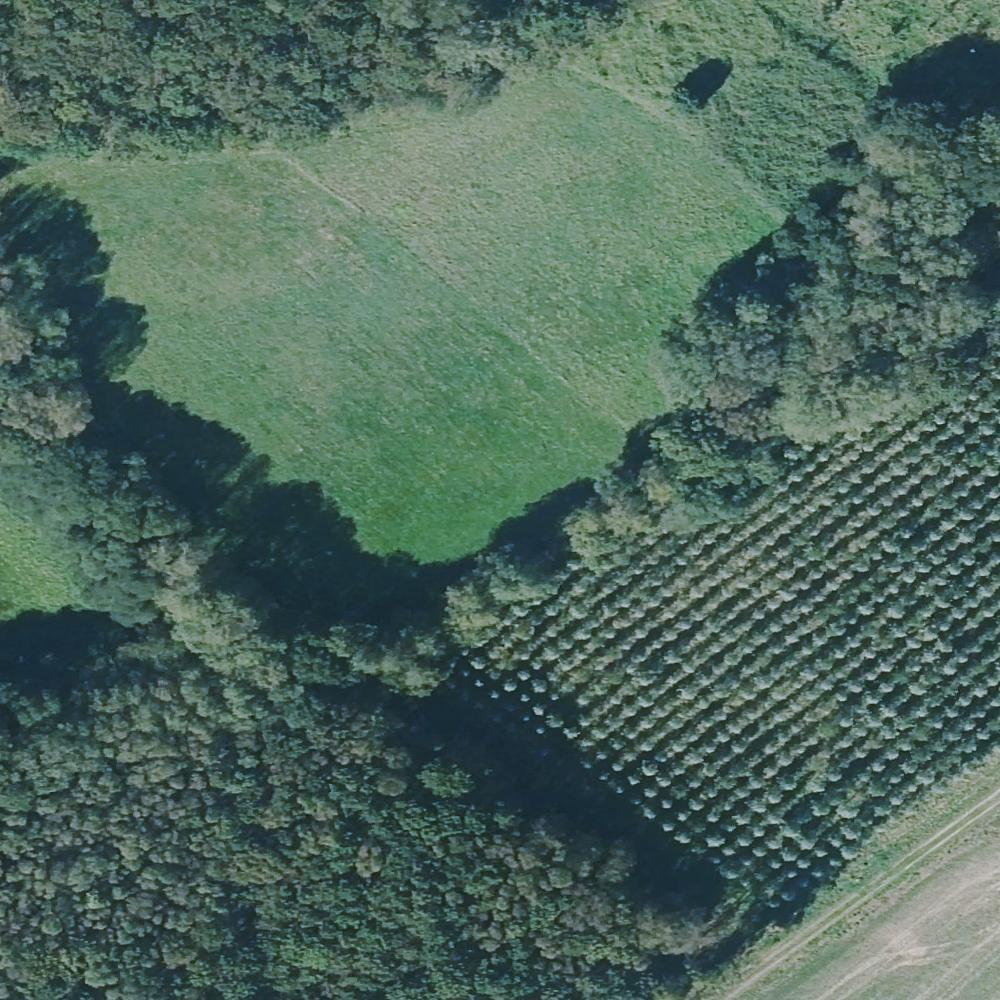
\includegraphics[width=\linewidth]{figuras/15_1903_1997.0.jpg}
        \label{fig:orto1}
    \end{subfigure}
    \hfill
    \begin{subfigure}[b]{0.31\textwidth}
        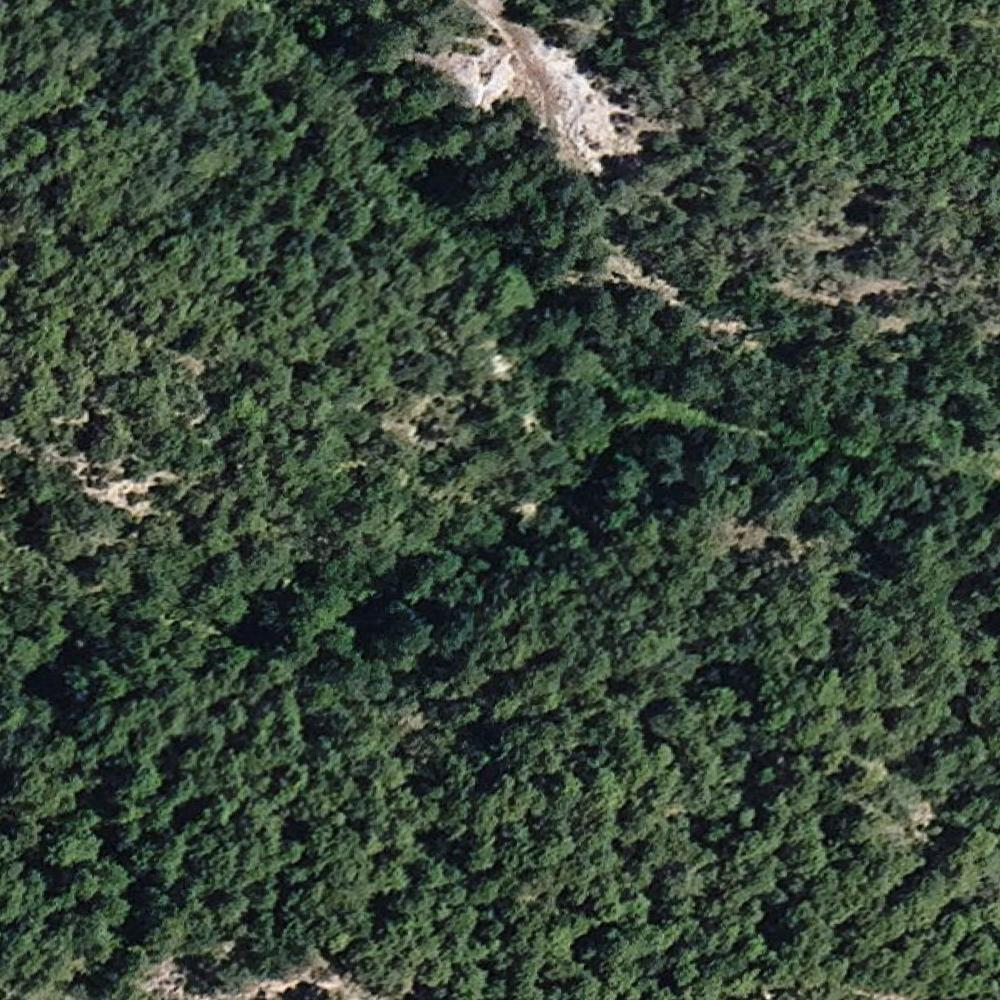
\includegraphics[width=\linewidth]{figuras/25_2209_2001.0.jpg}
        \label{fig:orto2}
    \end{subfigure}
    \hfill
    \begin{subfigure}[b]{0.31\textwidth}
        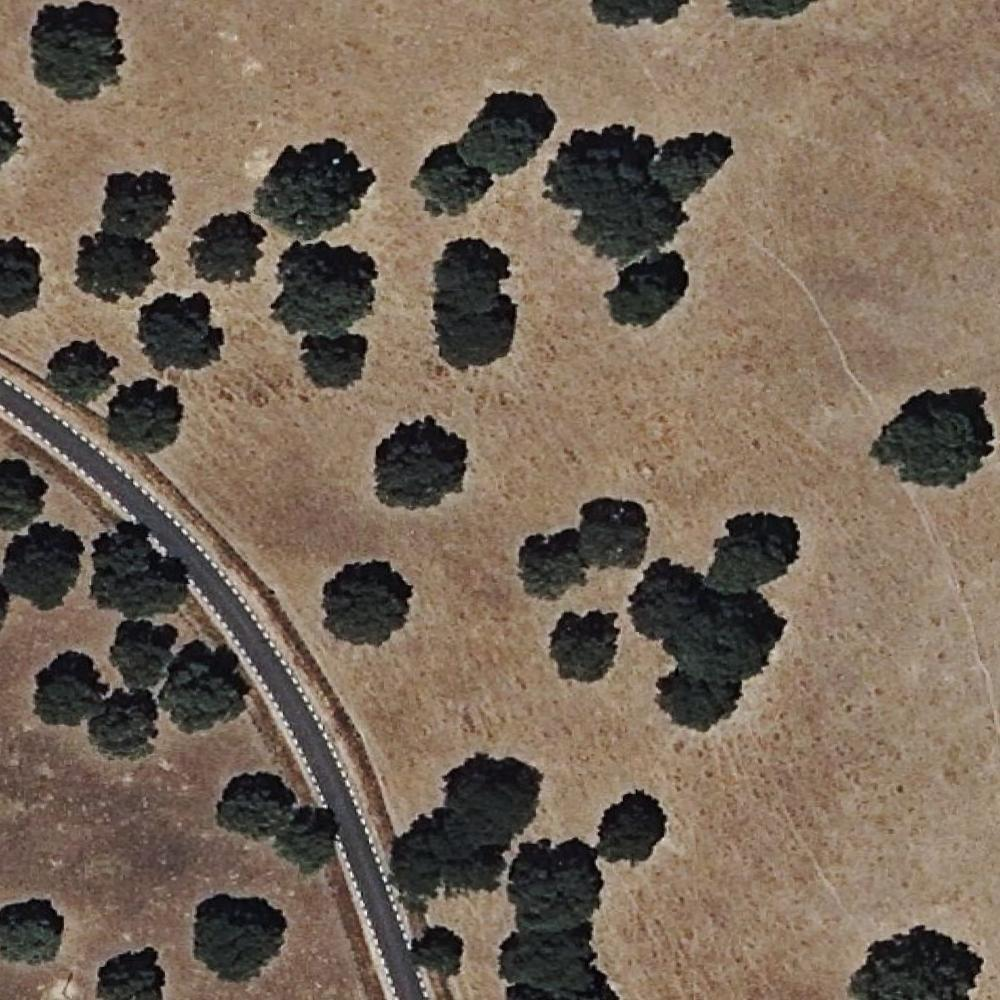
\includegraphics[width=\linewidth]{figuras/37_688_2002.0.jpg}
        \label{fig:orto3}
    \end{subfigure}
    
    \caption{\small Ejemplos de ortofotos del PNOA para tres parcelas del IFN. Se observa la cobertura arbórea y estructura del terreno con resolución submétrica. Estas imágenes fueron descargadas mediante peticiones WMS automatizadas en torno al centro geográfico de cada parcela.}
    \label{fig:ortofotos_ejemplo}
\end{figure}



\newpage
\section{Metodología de integración}

% Explica el proceso de construcción de la base de datos:
% - Cómo se alinearon las fuentes espacial y temporalmente
% - Procesos de limpieza, normalización o filtrado
% - Qué herramientas o lenguajes usaste (Python, QGIS, R, etc.)
% - Cómo se validó la integridad del conjunto de datos (valores faltantes, duplicados)
% - Cuál fue la lógica para estructurar los registros: por parcela, especie, clase diamétrica, etc.


La construcción de la base de datos se fundamenta en la integración de múltiples fuentes de información, alineadas espacial y temporalmente sobre una unidad básica común: la parcela del Inventario Forestal Nacional (IFN). Cada parcela está georreferenciada con coordenadas precisas, lo que permite su identificación única y la vinculación con otras capas de información espacial y temporal. Esta georreferenciación, junto con la fecha de muestreo (año de apeo), actúa como nexo de unión entre todos los conjuntos de datos empleados, posibilitando una articulación coherente y robusta de la información recopilada.

\medskip

Para cada una de las tres campañas del IFN consideradas (IFN2, IFN3 e IFN4), se toma el año de muestreo como referencia temporal. A partir de esta fecha se consulta, enlaza o calcula la información correspondiente de las demás fuentes. Así, por ejemplo, los datos meteorológicos y climáticos se extraen considerando el año anterior al muestreo, ya sea a nivel estacional o anual según la variable, mientras que las imágenes aéreas o satelitales se seleccionan para fechas cercanas al año de inventario. Esta estrategia garantiza que la información vinculada sea representativa del estado de la parcela en el momento del muestreo forestal.

\medskip

Desde el punto de vista técnico, el proceso de integración se llevó a cabo íntegramente en Python, apoyándose en bibliotecas como \texttt{pandas} y \texttt{geopandas} para la manipulación de datos tabulares y espaciales, \texttt{shapely} para el tratamiento geométrico, \texttt{owslib} y \texttt{PIL} para la descarga y procesamiento de imágenes aéreas, y \texttt{xarray} o \texttt{netCDF4} para la gestión de archivos climáticos multibanda. Adicionalmente, se emplearon herramientas SIG como QGIS de forma auxiliar para la validación visual de coberturas.

\medskip

La estructura de la base resultante se organiza jerárquicamente por parcela, inventario,  especie y clase diamétrica. Las tablas principales responden a claves compuestas que representan la identidad única de cada unidad de observación: \texttt{parcela}, \texttt{parcela\_inventario}, \texttt{parcela\_inventario\_especie} y \texttt{parcela\_inventario\_especie\_cd}. Además se incluye una tabla \texttt{parcela\_inventario\_estacion} en la que se almacenan los datos meteorológicos y satelitales de cada parcela que dependen de la estación. Durante el proceso de construcción se detectaron duplicidades en estas claves, causadas por errores de origen en los datos o repeticiones exactas. En una primera etapa se eliminaron todas las filas duplicadas completas. Posteriormente, para cada clave primaria compuesta, se retuvo únicamente el registro con menor número de valores ausentes (\texttt{NaN}), descartando los duplicados menos informativos.


\subsection{Preprocesado de los datos}

\subsubsection{Datos satelitales}

Todo el preprocesado de los datos satelitales se realiza con la herramienta \textit{Google Earth Engine}. A lo largo del preprocesamiento de los datos procedentes de satélites nos encontramos varios apartados. Para el caso de las imágenes:

\begin{itemize}
    \item \textbf{Eliminación de nubes y sombras, y enmascaramiento de los huecos}

    Con este paso tratamos de identificar y enmascarar píxeles que contienen nubes y sombras de nubes, los cuáles no nos dan información fiable sobre la superficie terrestre. Lo logramos seleccionando la banda de control de calidad QA\_PIXEL de la imagen, donde bits específicos indican la presencia de nubes (bit 5) y sombras de nubes (bit 3). Mediante operaciones lógicas bit a bit, cramos una máscara que marca como ``verdaderos'' (limpios) solo los píxeles libres de nubes y sombras. Finalmente, esta máscara se aplica a la imagen original, haciendo que las áreas afectadas por nubes y sombras se vuelvan transparentes o ``sin datos'', lo cual es esencial para asegurar análisis posteriores de la superficie terrestre sin interferencias atmosféricas. Un ejemplo de conjunto de datos para la primavera de $2004$ se puede ver en la Figura \ref{fig:imagenes_sat_primavera_2004}.

    \begin{figure}[H]
        \centering
        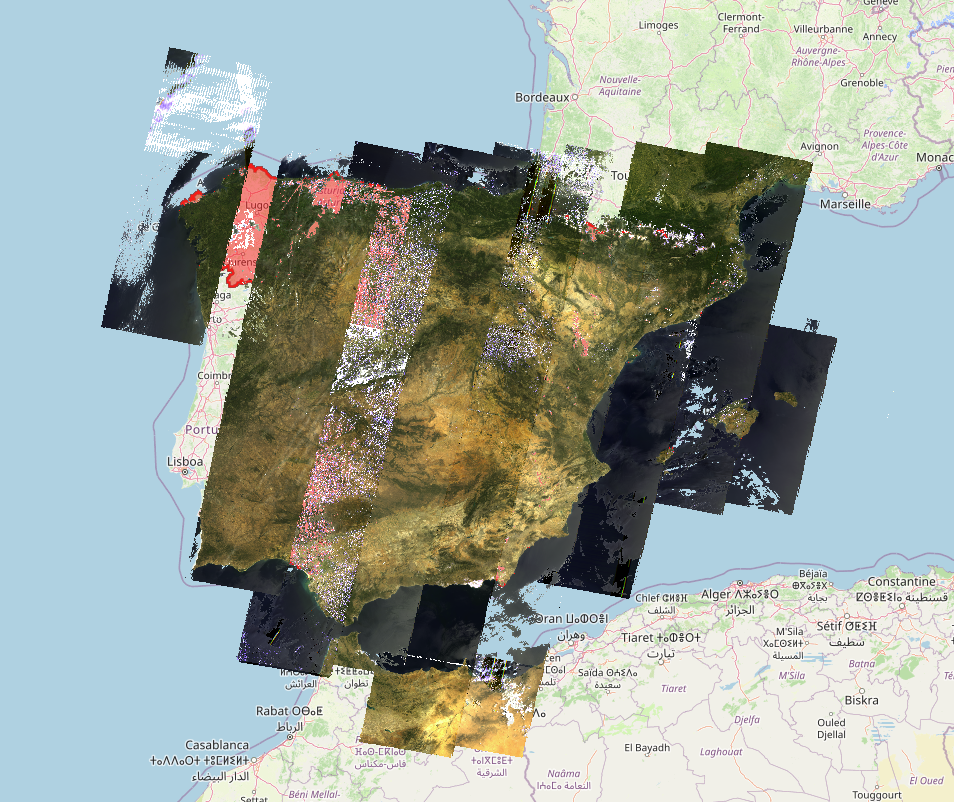
\includegraphics[width=0.7\linewidth]{figuras/ejemplo_imagen_sat_mala_calidad.png}
        \caption{Ejemplo de un conjunto de imágenes tras la eliminación de las nubes para la primavera de $2004$, que constituye un caso paradigmático del peor de los casos, en el que hay muchos huecos en las imágenes, para que se vea el procesado. Generalmente los datos son de mayor calidad (menos huecos) para el resto de años. Imágenes obtenidas del conjunto de datos Landsat 7 cortesía del Servicio Geológico de Estados Unidos.}
        \label{fig:imagenes_sat_primavera_2004}
    \end{figure}


    Si el periodo de observación que tomamos es relativamente corto (menos de 6 meses) y coincide con meses en los que suele haber más nubes, como es el otoño e invierno, nos encontraremos zonas en las que no tendremos observaciones, es decir, para una cierta zona no ha coincidido la pasada del satélite con un momento en el que no haya nubes. Para poder identificar estas zonas, identificaremos a estos puntos con el valor $-999$ para poder identificarlos claramente. También, para que esta situación se de lo menos posible, las imágenes de satélites las tomaremos solo para las estaciones de primavera y verano. 

    \item \textbf{Aplicación del factor de escala}

    La manera en la que están guardados los datos en el archivo original no representan directamente la reflectancia de la superficie o la temperatura en unidades físicas, principalmente por razones de eficiencia de almacenamiento, mantenimiento de precisión y similar. Para obtener valores con significado físico tenemos que aplicar una transformación lineal a los datos, la cuál podemos encontrar en la documentación del dataset, que es la siguiente:
    \begin{itemize}
        \item Transformación para las bandas ópticas (SR\_B):
        \[
        f(x) = 0.0000275x - 0.2.
        \]
        \item Transformación para las bandas térmicas (ST\_B6):
        \[
        f(x) = 0.00341802x + 149.
        \]
    \end{itemize}
    \item \textbf{Cálculo de los índices y otras medidas}\label{sec:indices}
    
    El siguiente paso es calcular los distintos índices vegetales que vamos a incorporar al modelo. Este proceso consiste en una serie de operaciones con algunas de las bandas del satélite según las longitudes de onda que éstas observen.

    \begin{itemize}
        \item \textbf{NDVI (Normalized Difference Vegetation Index)} \cite{eos_blog}
        
        El NDVI es uno de los más adecuados para seguir la dinámica de desarrollo de la vegetación, ya que mide la biomasa fotosintéticamente activa de las plantas. Sin embargo, este índice de vegetación es bastante sensible a la luminosidad del suelo y a los efectos atmosféricos, mitigados en otros índices como EVI.
        
        \[
        \text{NDVI} = \frac{\text{NIR} - \text{Red}}{\text{NIR} + \text{Red}} = \frac{\text{SR\_B4} - \text{SR\_B3}}{\text{SR\_B4} + \text{SR\_B3}}.
        \]
    
        \item \textbf{NDII (Normalized Index)} \cite{sentinel_hub_ndii}
        
        Es una medición de reflectancia, sensible a los cambios en el contenido de agua de los doseles vegetales. Los valores del índice aumentan con el incremento del contenido de agua. Las aplicaciones del NDII incluyen la gestión de cultivos agrícolas, el monitoreo de las copas de los árboles y la detección de vegetación estresada.
        \[
        \text{NDII} = \frac{\text{NIR} - \text{SWIR}}{\text{NIR} + \text{SWIR}} = \frac{\text{SR\_B4} - \text{SR\_B5}}{\text{SR\_B4} + \text{SR\_B5}}.
        \]
    
        \item \textbf{GNDVI (Green Normalized Difference Vegetation Index) } \cite{eos_indices_vegetacion}
        
        El índice GNDVI es una modificación del NDVI que también utiliza el infrarrojo cercano, pero sustituye el verde visible por el rojo visible. Suele emplearse para detectar cultivos marchitos o envejecidos y medir el contenido de nitrógeno en las hojas cuando no se dispone de un canal rojo extremo, monitorizar la vegetación con copas densas o en las etapas de madurez.
        \[
        \text{GNDVI} = \frac{\text{NIR} - \text{GREEN}}{\text{NIR} + \text{GREEN}} = \frac{\text{SR\_B4} - \text{SR\_B2}}{\text{SR\_B4} + \text{SR\_B2}}.
        \]
    
        \item \textbf{EVI (Enhanced Vegetation Index)} \cite{eos_indices_vegetacion}
        
        Se creó para ajustar los resultados del NDVI a los ruidos atmosféricos y del suelo, especialmente en las zonas de vegetación densa, así como para mitigar la saturación en la mayoría de los casos.
        
        \begin{align}
             \text{EVI} &= 2.5 \left( \frac{\text{NIR} - \text{RED}}{\text{NIR} + C_1 \cdot \text{RED} - C_2 \cdot \text{BLUE} + L} \right ), \\
             & = 2.5 \left( \frac{\text{SR\_B4 - SR\_B3}}{\text{SR\_B4} + C_1 \cdot \text{SR\_B3} - C_2 \cdot \text{SR\_B1 + L}} \right),
        \end{align}
   
        donde \(C_1 = 6\), \(C_2 = 7.5\) y \(L = 1\). El índice EVI contiene los coeficientes \(C_1\) y \(C_2\) para corregir la dispersión de los aerosoles presentes en la atmósfera y \(L\) para ajustar el fondo del suelo y las copas de la vegetación.
    
        \item \textbf{SLOPE (Pendiente)} \cite{ee_terrain_slope}
        
        Partiendo de un Mapa Digital de Terreno (DEM, por sus siglas en inglés) el gradiente local se calcula utilizando los 4 vecinos conectados de cada píxel, por lo que se producirán valores faltantes alrededor de los bordes de una imagen. El cálculo se realiza mediante la función \texttt{ee.Terrain.slope} de \textit{Google Earth Engine}.
    
        \item \textbf{ASPECT (Orientación)} \cite{ee_terrain_slope}
        
        De igual forma que para el caso anterior, este dato se calcula a partir de Mapa Digital de Terreno calculando el gradiente utilizando los 4 vecinos conectados de cada píxel. Se empleó la función \texttt{ee.Terrain.aspect} de \textit{Google Earth Engine}.
    \end{itemize}
\end{itemize}

Una vez realizado este proceso solo quedaría extraer el valor para las latitudes y longitudes que deseemos. 


\subsubsection{Inventario Forestal Nacional}

El objetivo de los siguientes pasos es la criba de los datos, eliminación e imputación de faltantes y la generación de identificadores únicos para las entradas de cada tabla. Tras este preprocesamiento se obtienen cuatro tablas con sus correspondientes identificadores únicos y con datos cribados. Se normalizan los códigos de las especies, se completan datos como las etiquetas de carbono y se estima la superficie de cada parcela.


\begin{itemize}
    \item \textbf{Creación de identificadores para cada tabla.} Para facilitar el manejo de los datos lo primero que se hace es crear un identificador para cada parcela. Esto se lleva a cabo concatenando \texttt{Estadillo} y \texttt{Provincia}. Este identificador debe tratarse con mucha atención pues es lo que permitirá relacionar las observaciones de uno y otro inventario. A partir de esta clave se construyen las claves primarias de cada tabla que deben ser tratadas para asegurar su unicidad: \texttt{idparcela\_inventario}, \texttt{idparcela\_inventario\_especie} e \texttt{idparcela\_inventario\_especie\_cd}.
    
    \medskip
    
    \item \textbf{Normalización de los códigos de las especies.} Se normaliza la codificación de las especies para que coincidan entre inventarios siguiendo la Tabla \ref{tab:codificacion_especies}. 

    
    \medskip

    \item \textbf{Filtrado por las coordenadas de las parcelas. } Eliminamos las parcelas que no tengan unas coordenadas válidas ($\texttt{CoorX}, \texttt{CoorY} =0$ o faltante). Consideramos dos parcelas como coincidentes entre dos inventarios cuando  tienen un mismo \texttt{idparcela} y sus coordenadas (tanto en X como en Y) estan a una distancia inferior a $300$m. Eliminamos las parcelas que no estén en al menos dos inventarios. Las coordenadas de los inventarios son progresivamente más precisas, siendo las coordenadas del cuarto inventario las mejores. Como, una vez filtradas, se considera una única ubicación para cada parcela, empleamos las coordenadas del inventario cuarto por defecto. En caso de no existir se emplean las coordenadas del inventario tercero, nunca las del segundo. 

    \medskip
    
    \item \textbf{Corrección en el huso geográfico.} Al proyectar las coordenadas de las parcelas sobre el mapa encontramos muchos errores (parcelas sobre el mar, en otros países o sobre la provincia equivocada). Tras la exploración de los datos encontramos que los errores se deben a una mala asignación de los husos geográficos. Vemos en la figura \ref{fig:husos} estas divisiones del territorio. 
    \begin{figure}[H]
        \centering
        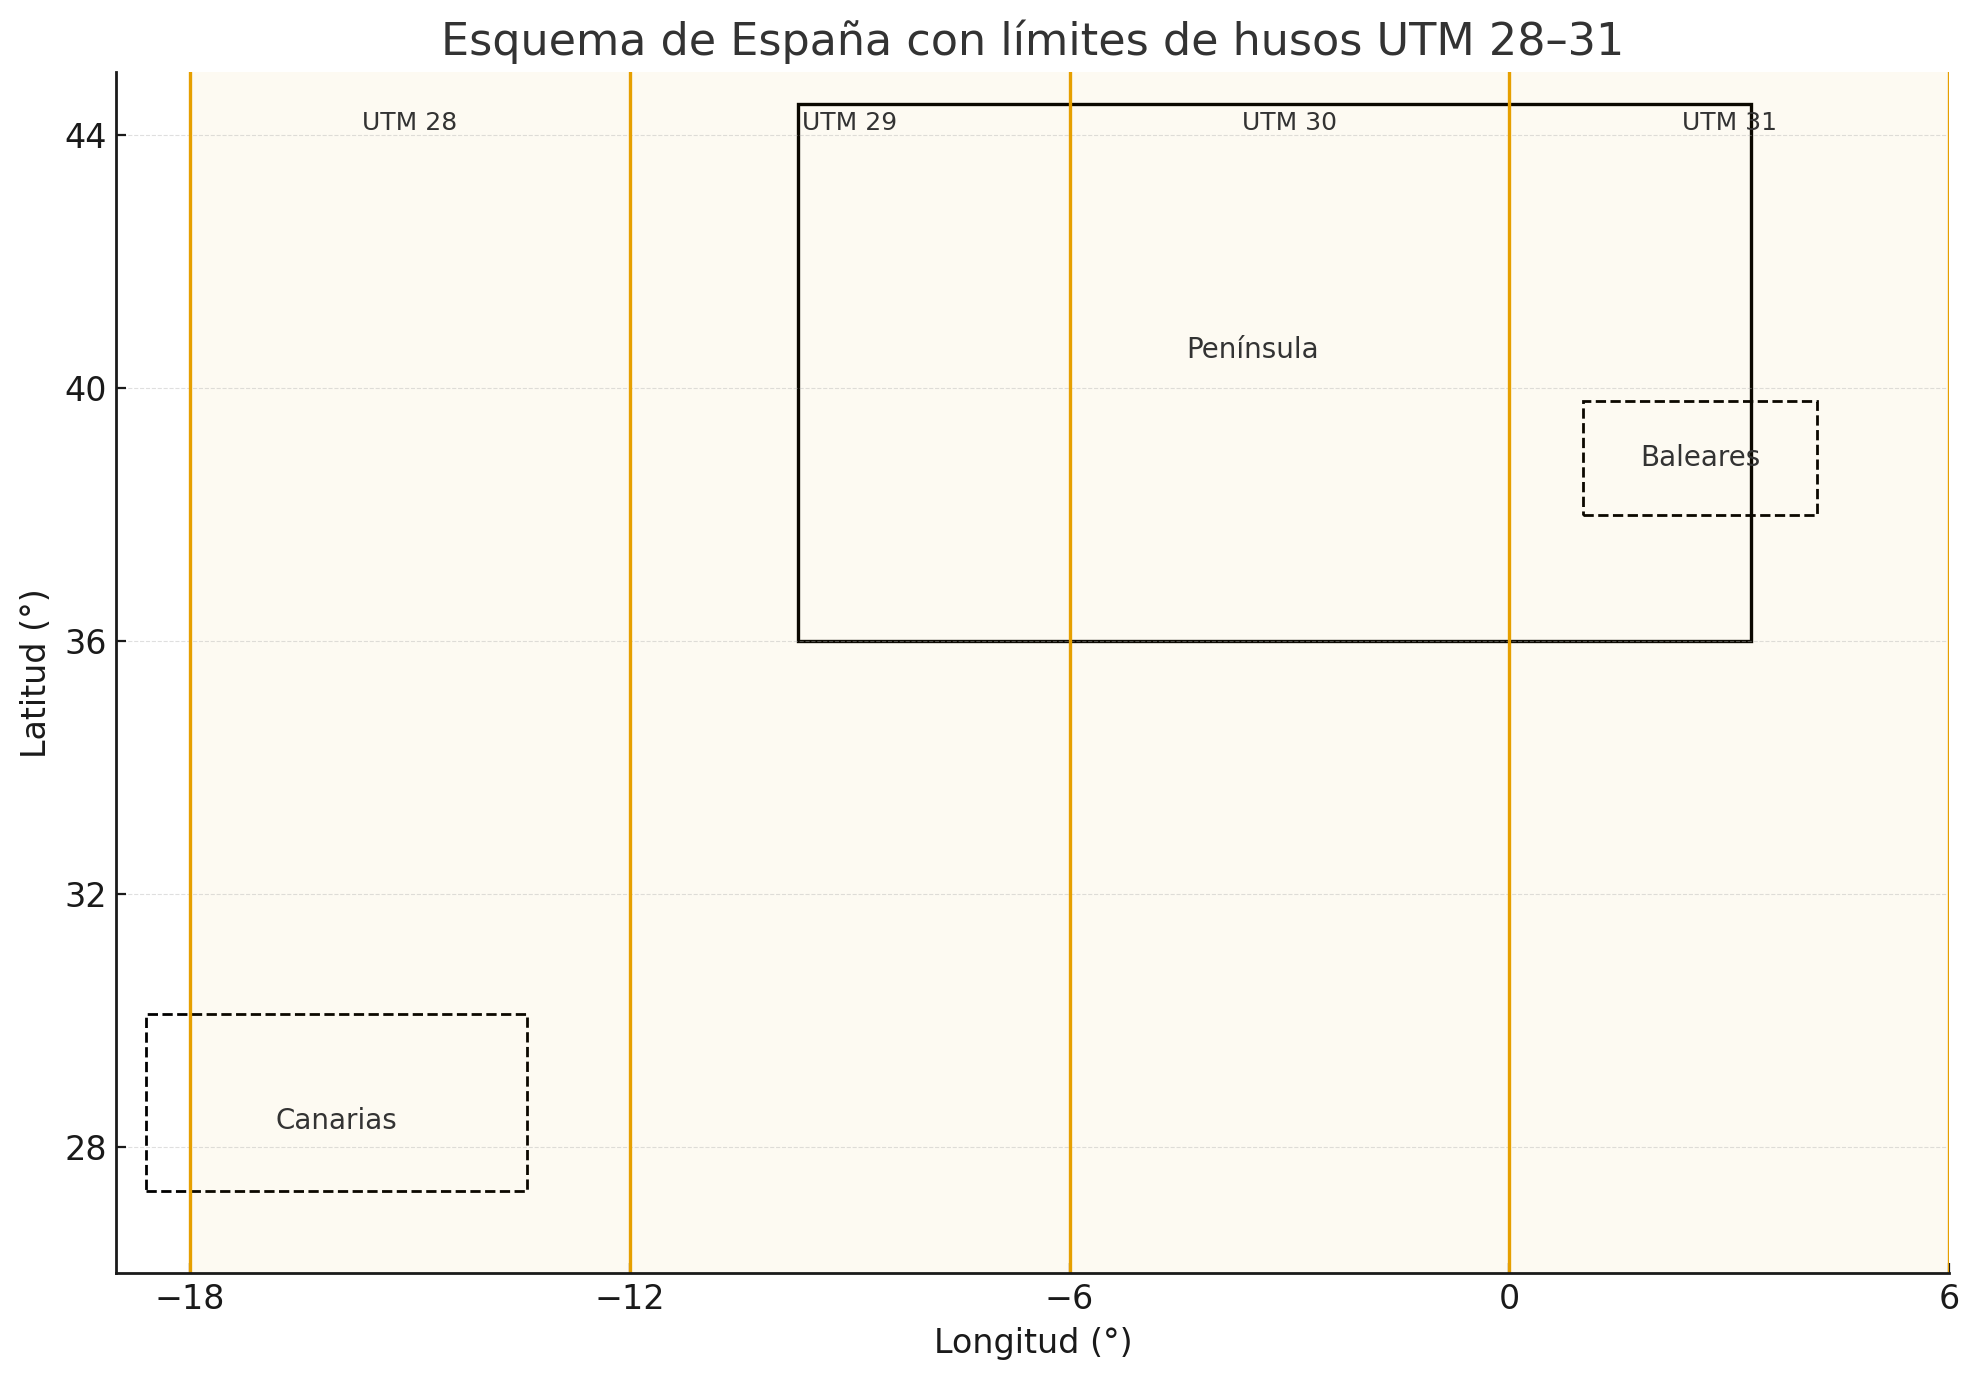
\includegraphics[width=0.4\textwidth]{figuras/husos.jpeg}
        \caption{\small Imagen del mapa peninsular con los husos geográficos. Se contemplan las bandas de huso 29, 30 y 31. Las islas Canarias no aparecen en la imagen pero sí que se contemplan en la base de datos (huso 28 y 29).}
        \label{fig:husos}
    \end{figure}
    
    Algunas de las provincias atravesadas por una de estas limitaciones geográficas mantienen el mismo valor de \texttt{Huso} para todas sus parcelas, no adaptandose al cambio en la proyección. Para identificar las parcelas mal proyectadas empleamos el \textbf{shapefile de la Base de Datos de Divisiones Administrativas de España} \cite{ign_shapefile}, de donde podemos obtener un rango en longitud y altitud de cada provincia. Corregimos el huso de aquellas parcelas cuya longitud esta fuera del rango de longitud de su provincia (la corrección es sencilla porque sabiendo cual es la provincia sabemos que frontera de huso la atraviesa). Eliminamos las parcelas que, una vez corregidas, tienen una longitud o latitud fuera de los rangos del territorio español. 

    \medskip

    \item \textbf{Filtrado por año de exploración.} Se eliminan los registros de las parcelas (entradas de las tablas cuya clave primaria contiene el inventario) anteriores a 1950. No existen datos de satélite para estos años y se sospecha que la mayoría de estas observaciones son erróneas. 

    \medskip
    
    \item \textbf{Incorporación de pies menores a \texttt{parcela\_inventario\_especie\_cd}.} Los datos de la tabla \texttt{brotes} (\ref{tab:brotes}) permiten identificar y caracterizar los cultivos forestales en su fase inicial. Esta tabla, como se puede consultar en el anexo \ref{sec:CatDesDensidad}, incluye un recuento de los especímenes de entre $30$ cm y $1,3$ m o aquellos de altura superior pero diámetro del tronco inferior a $7,5$ cm. Sin embargo, el recuento de pies por clase diamétrica incluido en la tabla \texttt{parcela\_inventario\_especie\_cd} (Tabla \ref{tab:parcela_inventario_especie_cd}) parten de una clase diamétrica igual a $10$ cm. Los datos de la tabla \texttt{brotes} se incorporan a la tabla \texttt{parcela\_inventario\_especie\_cd} (tabla \ref{tab:parcela_inventario_especie_cd}) de la siguiente manera: 
    
    \medskip
    
    Cada entrada de la tabla \texttt{brotes} corresponde a un conjunto de árboles de una parcela, inventario y especie concreta y se caracteriza por la variable \texttt{CatDes} o categoría del desarrollo: 
    
    \begin{enumerate}
        \item Pies con altura inferior a $30$ cm.
        \item Pies con altura comprendida entre $30$ y $130$ cm.
        \item Pies con altura superior a 130 cm y diámetro normal menor de $2,5$ cm.
        \item Pies con altura superior a $130$ cm y diámetro normal comprendido entre $2,5$ y $7,5$ cm. Corresponde a los pies menores del IFN2.
    \end{enumerate}
    
    \medskip
    
    Para añadir dichas entradas a la tabla \texttt{parcela\_inventario\_especie\_cd} (Tabla \ref{tab:parcela_inventario_especie_cd}) es necesario definir una clase diamétrica y estimar un número de pies para cada entrada/grupo de árboles. Mapeamos la variable \texttt{CatDes} a la clase diamétrica: Los valores de categoría del desarrollo $1$ y $2$ se asignan como \texttt{CD}$=1$, los valores $3$ se asignan como \texttt{CD}$=2$ y los valores $4$ se asignan como \texttt{CD}$=5$. 
    
    \medskip
    
    El número de árboles de cada grupo se extrae de la variable \texttt{Densidad}, esta se cuantifica según la categoría de desarrollo:
    
    \medskip
    
    \textbf{Para las categorías $1, 2$ y $3$}:
    \begin{enumerate}
        \item \textbf{Escasa:} De $1$ a $4$ pies en la parcela.
        \item \textbf{Normal:} De $5$ a $15$ pies en la parcela.
        \item \textbf{Abundante:} Más de $15$ pies en la parcela.
    
    \medskip
    
    \end{enumerate}
    \textbf{Para la categoría 4:}
    \begin{itemize}
        \item Se cuenta el número exacto de pies por especie en la subparcela de 5 m de radio. Se registra en la casilla ``NPies''.
    \end{itemize}
    
    \medskip
    
    Así, se ajusta el número de árboles de cada grupo según el valor de \texttt{Densidad}. Si el valor de \texttt{Densidad} es 1, 2 o 3, se asignan valores específicos a \texttt{NPies} (2.5, 10 y 15, respectivamente); de lo contrario, se conserva el valor original de \texttt{NumPies}.
    
    \medskip

    \item \textbf{Variables \texttt{CA} y \texttt{CR}.} Estas variables (carbono arbolado y carbono radical por hectárea\footnote{Diferenciamos entre la fijación de carbono aéreo del arbolado y la fijación de carbono radical del arbolado, dos componentes distintos del almacenamiento total de carbono en un ecosistema forestal. La fijación de carbono aéreo se refiere a la cantidad de carbono almacenado en la biomasa aérea del arbolado (tronco, ramas, hojas) y la fijación de carbono radical a la cantidad de carbono almacenado en el sistema radical (raíces); representan el 70-80\% y el 20-30\% del carbono total del árbol respectivamente. Ambos son relevantes, pero el carbono aéreo es el más comúnmente contabilizado en proyectos de créditos de carbono por ser más fácil de contabilizar y de asegurar su permanencia. }) están registradas solo para el IFN4 para cada grupo de árboles de una clase diamétrica y especie concreta (tabla \texttt{parcela\_especie\_inventario\_cd} (\ref{tab:parcela_inventario_especie_cd}) restringida al inventario cuarto) y se calculan usando la Guía para la estimación de absorciones de dióxido de carbono propuesta por el MITECO \cite{miteco_guia_co2}. 

    \medskip

    Algunas provincias (las provincias $07, 15, 27, 30, 31, 32, 33, 36, 39$ y del País Vasco) no tienen las variables \texttt{CA} y \texttt{CR} registradas por lo que es necesario estimarlas. Para solucionar estos faltantes, además de los debidos a fallos en la recogida de los datos, se emplea un  modelo \textit{RandomForestRegressor}
\footnote{Para evaluar el modelo se dividen los datos en un $80\%$ para entrenamiento y un $20\%$ para validación. El modelo para \texttt{CA} obtiene: $\text{MSE}_{\text{CA, train}}= 0.28$, $\text{MSE}_{\text{CA, test}} = 5.48$, $R^2_{\text{CA, train}} = 0.99$, $R^2_{\text{CA, test}} = 0.91$. Para \texttt{CR}, las métricas son: $\text{MSE}_{\text{CR, train}}= 0.24$, $\text{MSE}_{\text{CR, test}}= 1.34$, $R^2_{\text{CR, train}} = 0.99$, $R^2_{\text{CR, test}} = 0.94$.}
, que permite predecir estos valores a partir de las características disponibles en los datos. El modelo se entrena utilizando un conjunto de variables predictoras, que incluyen \texttt{Especie,  CD, VSC, NPies, ABas, IAVC, VCC} y \texttt{VLE}. Este mismo modelo se aplica para asignar etiquetas de carbono a los datos del inventario tercero y segundo (IFN2 e IFN3). Los datos provenientes de la tabla \texttt{brotes} (Tabla \ref{tab:brotes}) se consideran de carbono $0$. 

\medskip

\item \textbf{Creación de la variable \texttt{c} (carbono).} Creamos la variable \texttt{c} que será la variable objetivo del modelo como \texttt{c=CA+CR} para cada entrada de la tabla \texttt{parcela\_inventario\_especie\_cd} (tabla \ref{tab:parcela_inventario_especie_cd}). Los valores de estas variables se registran en toneladas por hectárea y, por tanto, para generalizar a las entradas de la tabla \texttt{parcela\_inventario\_especie} (Tabla \ref{tab:parcela_inventario_especie}) solo se requiere agrupar en \texttt{parcela\_inventario\_especie\_cd} por especie y sumar los valores de \texttt{c}.

\item \textbf{Filtrado por valores de \texttt{c} y número de árboles.} Se eliminan de la base de datos las parcelas que no registran carbono capturado en ningún inventario (\texttt{c} igual a 0 en IFN2, IFN3 e IFN4). Además, se eliminan las especies de las parcelas que no tienen registro en ninguno de los inventarios de la presencia de árboles (aquellos valores de \texttt{parcela\_inventario\_especie} no presentes en \texttt{parcela\_inventario\_especie\_cd}). 

\medskip

\item \textbf{Estimación de la superficie de la parcela.} El IFN no proporciona las dimensiones de cada parcela registrada. Para estimar este dato empleamos la variable \texttt{Distanci} de la tabla parcela (\ref{tab:parcela}). Las coordenadas de cada parcela registran el punto central de la parcela y de la documentación de los inventarios se entiende que se trata de parcelas circulares. La variable \texttt{Distanci} registra un conjunto de medidas correspondientes a la distancia entre cada pie mayor contenido en la parcela y el centro de la misma. Estimamos el radio de la parcela como la mayor de dichas distancias (distancia entre el centro de la parcela y el árbol más alejado contenido en ella). Registramos las variables \texttt{Radio} en metros y la variable \texttt{Superficie} en hectáreas. Las parcelas que no cuentan con mediciones de \texttt{Distanci} validas se imputan con la media. 
 
\end{itemize}


\newpage
\section{Estructura de la base de datos}

% Incluye:
% - Una lista de variables con sus nombres, unidades y descripciones
% - Qué tipo de datos contiene cada campo (numérico, categórico, geográfico)
% - Cuántos registros hay, si hay valores faltantes, etc.
% Puedes presentar una tabla con:
% | Variable | Descripción | Unidad | Tipo de dato |

La base de datos se organiza bajo un modelo relacional normalizado que garantiza la integridad referencial y la trazabilidad de los datos. Todas las claves primarias (\textit{PK}) están definidas explícitamente y siguen una nomenclatura uniforme terminada en \texttt{\_id}, representando la granularidad del dato en cada nivel jerárquico. De igual forma, las claves foráneas (\textit{FK}) se encuentran activas y estrictamente validadas, cubriendo el 100\% de los valores no nulos y asegurando la ausencia de registros huérfanos.

El esquema se ha diseñado para ser evolutivo y auditable. Las relaciones principales (PK/FK) permanecen estables, mientras que las tablas son extensibles, permitiendo incorporar nuevas métricas sin comprometer la coherencia estructural. La tabla \texttt{meta\_variables} complementa esta arquitectura documentando el tipo, unidades, método de cálculo, rango esperado y fuente de cada variable, lo que facilita la trazabilidad analítica y la reproducibilidad de los resultados.

\subsection*{Panorama de entidades}

Las tablas se agrupan en dos conjuntos: \textbf{núcleo} y \textbf{catálogos}.  
El núcleo contiene las entidades troncales que almacenan la información principal del sistema, mientras que los catálogos definen dominios controlados para las variables categóricas, garantizando consistencia terminológica en toda la base de datos.

\paragraph{Núcleo}
\begin{itemize}
  \item \textbf{parcelas}: identifica la unidad espacial (\texttt{parcela\_id}) y almacena su geometría básica (coordenadas, superficie, elevación, pendiente, etc.). Es la entidad raíz del modelo.
  \item \textbf{parcela\_inventario}: describe el estado de cada parcela en un inventario determinado (\texttt{parcela\_id}, \texttt{inventario\_id}), incluyendo atributos edáficos y de contexto (p. ej., \texttt{nivel1\_id}, \texttt{textura\_id}).
  \item \textbf{parcela\_inventario\_especie}: detalla la presencia y condición de cada especie dentro de una parcela e inventario, incorporando descriptores de masa y tratamientos silvícolas.
  \item \textbf{parcela\_inventario\_especie\_cd}: describe las poblaciones arbóreas por parcela, especie y \emph{clase diamétrica} (\texttt{cd\_id}): n.º de pies (\texttt{npies}), área basimétrica (\texttt{abas}), volúmenes (\texttt{vcc}, \texttt{vsc}, \texttt{vle}), incrementos (\texttt{iavc}) y carbono (\texttt{ca}, \texttt{cr}).
  \item \textbf{parcela\_especie\_arbol}: caracteriza los pies mayores identificados por parcela y especie en el inventario cuarto. Recoge las caracteristicas particulares de cada pie como altura (\texttt{ht}), diámetros (\texttt{dn1} y \texttt{dn2}), ubicación respecto del centro de la parcela (\texttt{rumbo}, \texttt{distancia}), volumen (\texttt{vcc, vsc, vle}), incremento (\texttt{iavc}) y carbono (\texttt{ca, cr}).  
  \item \textbf{parcela\_inventario\_estacion}: almacena agregados climático-biofísicos por estación (\texttt{estacion\_id}) en la misma granularidad parcela–inventario, incluyendo variables como precipitación (\texttt{PR}) y temperatura (\texttt{T2M, SKT, STL*}), junto a índices de vegetación (NDVI, EVI, NDII, GNDVI).
  \item \textbf{especies} y \textbf{grupos}: recogen la información taxonómica y su clasificación jerárquica, estableciendo la relación entre especies individuales y grupos funcionales.
\end{itemize}

\paragraph{Catálogos}
Cada variable categórica posee una tabla de catálogo propia (\texttt{cat\_}), donde se definen los valores posibles y sus descripciones. Por ejemplo, \texttt{cat\_textura}, \texttt{cat\_nivel1}, \texttt{cat\_tratmasa} o \texttt{cat\_origen}. Todas siguen un patrón uniforme: la clave primaria es el identificador de la variable (\texttt{<variable>\_id}), y las tablas núcleo referencian este mismo campo como clave foránea. Esto permite mantener un dominio controlado y una semántica coherente en toda la base de datos.

\subsection*{Representación del esquema}

La Figura~\ref{fig:GWest_BBDD} muestra el esquema general de las tablas nucleares y sus principales relaciones. Este diagrama resume la estructura interna de la base de datos y su jerarquía de dependencias.

\begin{figure}[H]
  \centering
  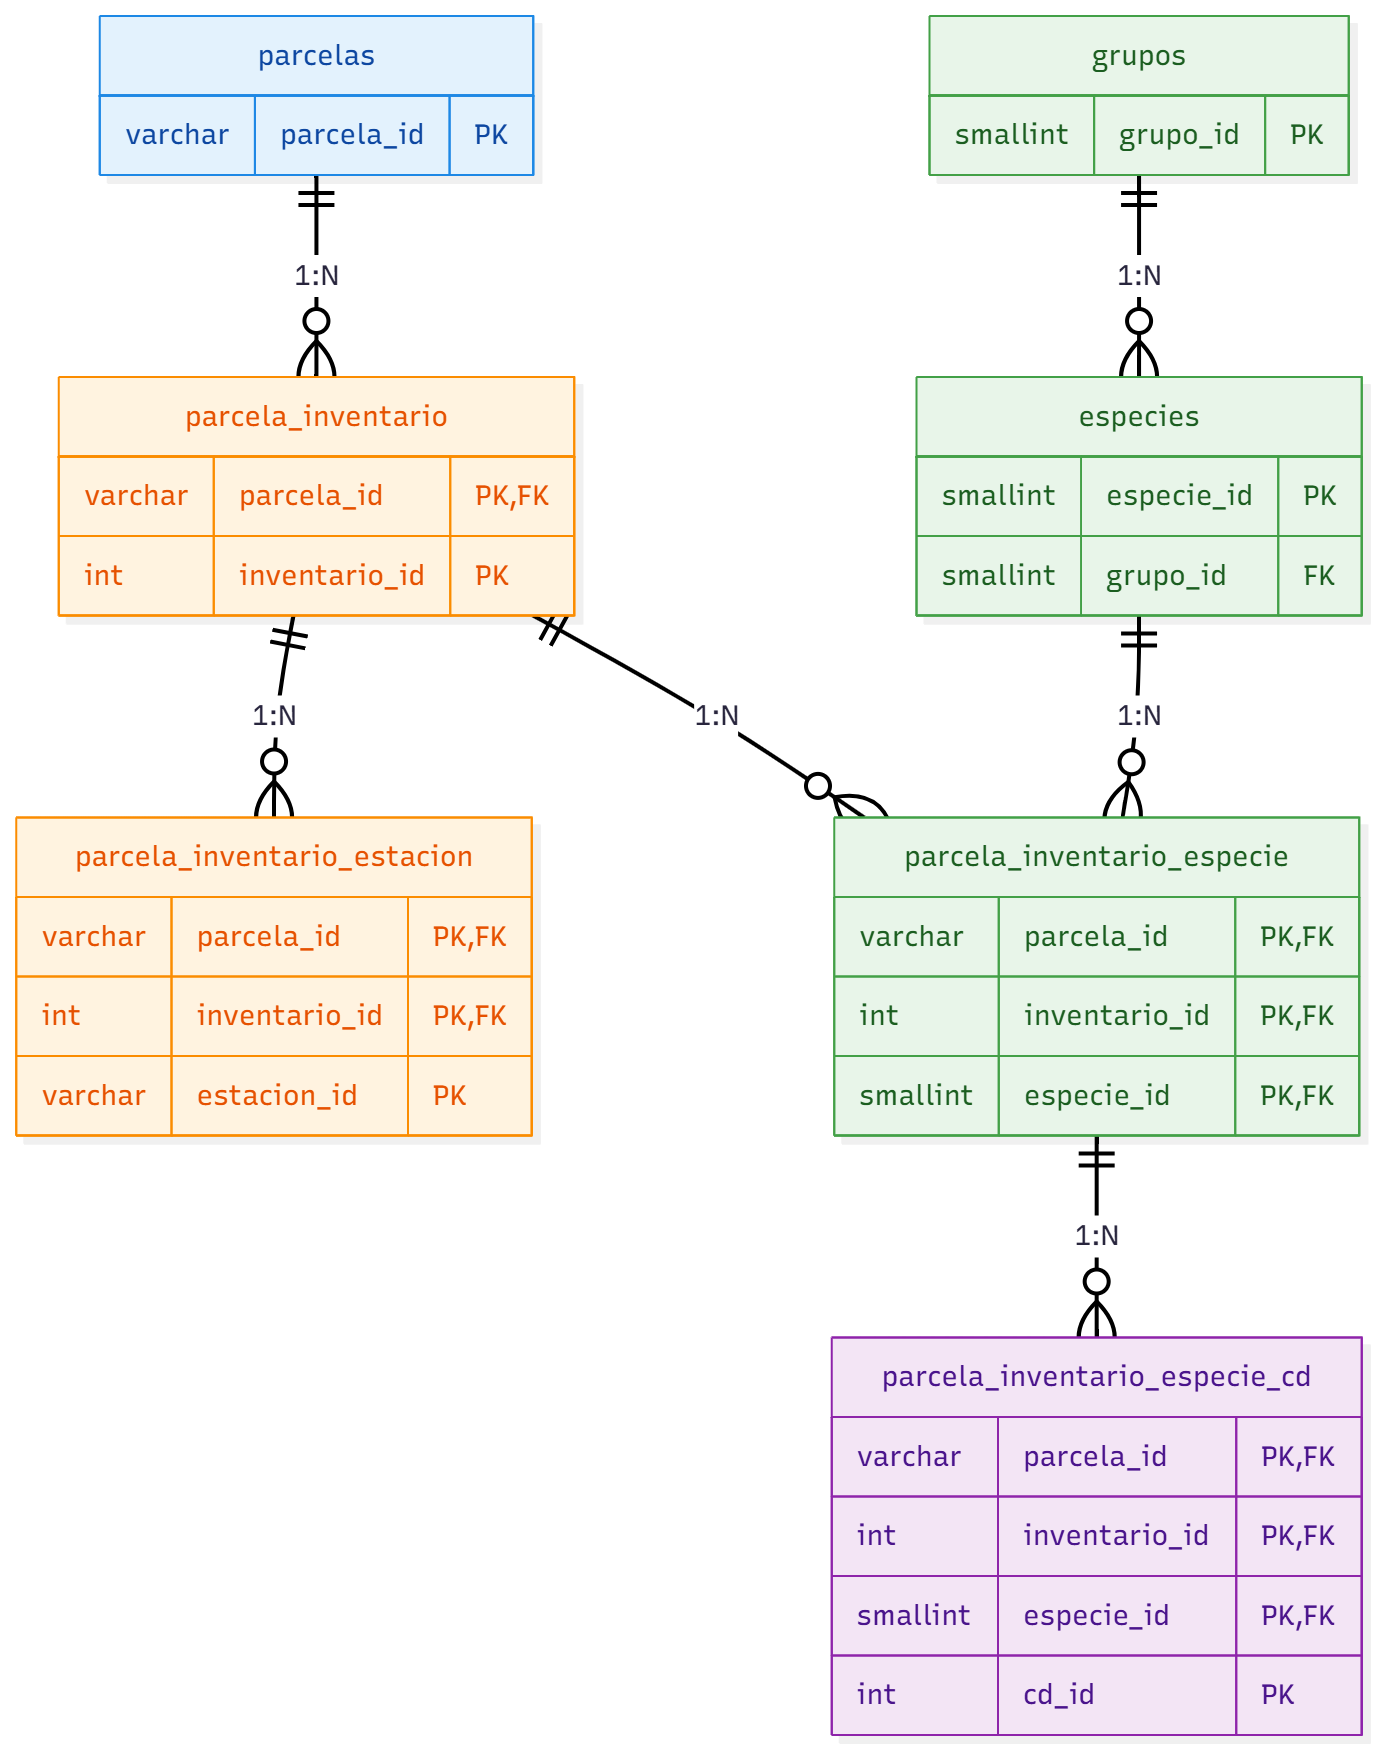
\includegraphics[width=0.9\textwidth]{figuras/Estrctr_BBDD_GWest.png}
  \caption{Esquema relacional de las tablas nucleares de la base de datos.}
  \label{fig:GWest_BBDD}
\end{figure}

\subsection*{Tipología de datos y convenciones}

Cada columna se tipifica en una de cuatro categorías:
\begin{itemize}
  \item \textbf{Numérico}: magnitudes continuas (p.\,ej., \texttt{npies}, \texttt{vcc}, \texttt{ndvi\_mean}, \texttt{elevacion}).
  \item \textbf{Categórico}: códigos discretos con dominio controlado mediante catálogos \texttt{cat\_*} (p.\,ej., \texttt{nivel1\_id}, \texttt{textura\_id}, \texttt{tratmasa\_id}).
  \item \textbf{Identificador}: claves primarias y foráneas terminadas en \texttt{\_id} (p.\,ej., \texttt{parcela\_id}, \texttt{inventario\_id}, \texttt{especie\_id}, \texttt{cd\_id}).
  \item \textbf{Geográfico}: coordenadas y derivados topográficos (\texttt{latitud}, \texttt{longitud}, \texttt{coorx}/\texttt{coory}, \texttt{pendiente}, \texttt{orientacion}).
\end{itemize}

Las variables satelitales y climáticas usan convenciones de \emph{valores especiales} para datos no disponibles o enmascarados por calidad (\texttt{NA}); los rangos esperados se documentan en \texttt{meta\_variables}. Todas las claves categóricas referencian explícitamente su catálogo homólogo (\texttt{<variable>\_id} $\rightarrow$ \texttt{cat\_<variable>(<variable>\_id)}).

\subsection*{Cardinalidad y completitud}

El volumen actual por tabla es:
\begin{center}
\begin{tabular}{l r}
\toprule
\textbf{Tabla} & \textbf{Número de registros} \\
\midrule
\texttt{parcelas} & 52{,}298 \\
\texttt{parcela\_inventario} & 147{,}995 \\
\texttt{parcela\_inventario\_especie} & 417{,}119 \\
\texttt{parcela\_inventario\_especie\_cd} & 1{,}191{,}070 \\
\texttt{parcela\_especie\_arbol} & 855{,}860 \\
\texttt{parcela\_inventario\_estacion} & 470{,}056 \\
\texttt{especies} & 195 \\
\texttt{grupos} & 33 \\
\bottomrule
\end{tabular}
\end{center}

Las \textit{FK} estructurales están activas y cubren el 100\,\% de los valores no nulos (sin huérfanos). La completitud de campos numéricos puede verse afectada por enmascaramientos de calidad en series satelitales/climáticas, registrados como \texttt{NA} según \texttt{meta\_variables}. Las variables categóricas presentan dominios cerrados controlados por sus catálogos.

\subsection*{Diccionario resumido de variables (núcleo)}
\small
\setlength{\LTcapwidth}{\textwidth}
\begin{longtable}{p{3.2cm} p{7.6cm} p{2.4cm} p{2.4cm}}
\caption{Resumen de variables principales por entidad. El diccionario completo se encuentra documentado en \texttt{meta\_variables}.}\\
\toprule
\textbf{Variable} & \textbf{Descripción} & \textbf{Unidad} & \textbf{Tipo de dato} \\
\midrule
\endfirsthead
\toprule
\textbf{Variable} & \textbf{Descripción} & \textbf{Unidad} & \textbf{Tipo de dato} \\
\midrule
\endhead
\midrule
\multicolumn{4}{r}{\emph{Continúa en la siguiente página}} \\
\midrule
\endfoot
\bottomrule
\endlastfoot

\multicolumn{4}{l}{\textbf{parcelas}} \\
\texttt{parcela\_id} & Identificador único de parcela (IFN). & -- & Identificador \\
\texttt{latitud}, \texttt{longitud} & Coordenadas geográficas (WGS84). & ° & Geográfico \\
\texttt{coorx}, \texttt{coory} & Coordenadas UTM; \texttt{huso} especifica zona. & m (UTM) & Geográfico \\
\texttt{elevacion} & Cota sobre el nivel del mar (NASADEM). & m & Numérico \\
\texttt{pendiente} & Inclinación del terreno. & ° & Numérico \\
\texttt{orientacion} & Orientación del terreno (0–360). & ° & Numérico \\
\texttt{presencia\_id} & Presencia en IFN $\rightarrow$ \texttt{cat\_presencia}. & -- & Categórico \\
\texttt{tipsuelo1\_id}, \texttt{tipsuelo2\_id}, \texttt{tipsuelo3\_id} & Tipos de suelo $\rightarrow$ \texttt{cat\_tipsuelo*}. & -- & Categórico \\
\texttt{rocosidad\_id} & Rocosidad $\rightarrow$ \texttt{cat\_rocosidad}. & -- & Categórico \\
\texttt{radio}, \texttt{superficie} & Radio de parcela y superficie derivada. & m; ha & Numérico \\
\addlinespace

\multicolumn{4}{l}{\textbf{parcela\_inventario}} \\
\texttt{parcela\_id}, \texttt{inventario\_id} & Clave compuesta (parcela-inventario). & -- & Identificador \\
\texttt{ano} & Año de apeo. & año & Numérico \\
\texttt{nivel1\_id}, \texttt{nivel2\_id} & Morfoestructura. $\rightarrow$ \texttt{cat\_nivel*}. & -- & Categórico \\
\texttt{textura\_id} & Textura de suelo $\rightarrow$ \texttt{cat\_textura}. & -- & Categórico \\
\texttt{merosiva\_id} & Manifestaciones erosivas $\rightarrow$ \texttt{cat\_merosiva}. & -- & Categórico \\
\texttt{matorg\_id} & Materia orgánica $\rightarrow$ \texttt{cat\_matorg}. & -- & Categórico \\
\texttt{modcomb\_id} & Modelo de combustible $\rightarrow$ \texttt{cat\_modcomb}. & -- & Categórico \\
\texttt{disesp\_id} & Distribución espacial $\rightarrow$ \texttt{cat\_disesp}. & -- & Categórico \\
\texttt{comesp\_id} & Composición específica $\rightarrow$ \texttt{cat\_comesp}. & -- & Categórico \\
\texttt{fccarb}, \texttt{fcctot} & Fracción de cabida cubierta (árboles). & \% & Numérico \\
\addlinespace

\multicolumn{4}{l}{\textbf{parcela\_inventario\_especie}} \\
\texttt{parcela\_id}, \texttt{inventario\_id}, \texttt{especie\_id} & Clave compuesta (parcela-inventario-especie). & -- & Identificador \\
\texttt{ocupa} & Grado de ocupación de la especie. & (0--10) & Numérico \\
\texttt{estado\_id} & Estado de desarrollo. $\rightarrow$ \texttt{cat\_estado}. & -- & Categórico \\
\texttt{fpmasa\_id} & Forma principal de masa $\rightarrow$ \texttt{cat\_fpmasa}. & -- & Categórico \\
\texttt{tratmasa\_id} & Tratamientos selvícolas $\rightarrow$ \texttt{cat\_tratmasa}. & -- & Categórico \\
\texttt{orgmasa1\_id} & Origen de masa (IFN3/4)$\rightarrow$ \texttt{cat\_orgmasa1}. & -- & Categórico \\
\texttt{masa\_id} & Clasificación de masa $\rightarrow$ \texttt{cat\_masa}. & -- & Categórico \\
\texttt{origen\_id} & Origen de la masa (IFN2) $\rightarrow$ \texttt{cat\_origen}. & -- & Categórico \\
\addlinespace

\multicolumn{4}{l}{\textbf{parcela\_inventario\_especie\_cd}} \\
\texttt{parcela\_id}, \texttt{inventario\_id}, \texttt{especie\_id} & Clave compuesta ( parcela-inventario-especie-cd). & -- & Identificador \\
\texttt{cd\_id} & Clase diamétrica (CD) reglamento IFN. & cm & Numérico discreto \\
\texttt{npies} & Número de pies. & pies/ha & Numérico \\
\texttt{abas} & Área basimétrica. & m$^{2}$/ha & Numérico \\
\texttt{vcc}, \texttt{vsc}, \texttt{vle} & Volúmenes (con/sin corteza; leñas). & m$^{3}$/ha & Numérico \\
\texttt{iavc} & Incremento anual del volumen con corteza. & m$^{3}$/ha$\cdot$año & Numérico \\
\texttt{ca}, \texttt{cr} & Carbono aéreo y radical. & t/ha & Numérico \\
\texttt{ht} & Altura media (modelo CatBoost). & m & Numérico \\
\texttt{carbono\_bruto} & Carbono total estimado (alometrías). & t & Numérico \\
\addlinespace

\multicolumn{4}{l}{\textbf{parcela\_especie\_arbol}} \\
\texttt{parcela\_id}, \texttt{especie\_id} & Clave compuesta (parcela–especie–árbol). & -- & Identificador \\ 
\texttt{arbol\_id} & Identificador del árbol dentro de parcela y especie. & -- & Entero \\ 
\texttt{rumbo} & Rumbo desde el centro de la parcela al árbol. & grados centesimales & Numérico \\ 
\texttt{distancia} & Distancia desde el centro de la parcela al árbol. & m & Numérico \\ 
\texttt{cd} & Clase diamétrica (reglamento IFN). & cm & Numérico discreto \\ 
\texttt{ht} & Altura total del árbol inventariado. & m & Numérico \\ 
\texttt{dn1}, \texttt{dn2} & Diámetros normales perpendiculares. & mm & Numérico \\ 
\texttt{abas} & Área basimétrica del pie medido. & m$^{2}$ & Numérico \\ 
\texttt{iavc} & Incremento anual del volumen con corteza. & dm$^{3}$/año & Numérico \\ 
\texttt{vcc}, \texttt{vsc}, \texttt{vle} & Volúmenes (con corteza, sin corteza, leñas). & dm$^{3}$ & Numérico \\ 
\texttt{ca}, \texttt{cr} & Carbono aéreo y radical del árbol. & t & Numérico \\
\addlinespace

\multicolumn{4}{l}{\textbf{parcela\_inventario\_estacion}} \\
\texttt{parcela\_id}, \texttt{inventario\_id}, \texttt{estacion\_id} & Clave compuesta (agregado estacional). & -- & Identificador \\
\texttt{PR\_*} & Estadísticos de precipitación (mean, max, min, std, sum). & mm/(m$^2\cdot$día), mm/m$^2$ & Numérico \\
\texttt{T2M\_*}, \texttt{SKT\_*} & Aire 2\,m y temperatura superficial (mean, max, min, std). & °C & Numérico \\
\texttt{STL1\_*}--\texttt{STL4\_*} & Temperatura del suelo por niveles (mean, max, min, std). & °C & Numérico \\
\texttt{NDVI\_*}, \texttt{EVI\_*}, \texttt{NDII\_*}, \texttt{GNDVI\_*} & Índices de vegetación (max, mean, median, min, std). & adimensional & Numérico \\
\addlinespace

\multicolumn{4}{l}{\textbf{especies} y \textbf{grupos}} \\
\texttt{especie\_id} & Identificador de especie IFN. & -- & Identificador \\
\texttt{nombre}, \texttt{sinonimia} & Denominación IFN y sinónimos. & -- & Texto \\
\texttt{tipo\_especie} & 0\,= conífera; 1\,= frondosa. & -- & Categórico \\
\texttt{grupo\_id} & Grupo funcional $\rightarrow$ \texttt{grupos}. & -- & Identificador \\
\texttt{grupos.nombregrupo} & Nombre del grupo. & -- & Texto \\
\end{longtable}
\normalsize
\subsection*{Calidad de datos y valores faltantes}

Las validaciones automáticas garantizan:
\begin{enumerate}
  \item \textbf{Integridad referencial}: todas las \textit{FK} (\texttt{parcela\_id}, \texttt{inventario\_id}, \texttt{especie\_id} y catálogos \texttt{cat\_*}) están resueltas sin registros huérfanos.
  \item \textbf{Rangos y dominios}: se verifican contra \texttt{rango\_esperado} y \texttt{valores\_especiales} de \texttt{meta\_variables}.
  \item \textbf{Faltantes}: en variables derivadas de teledetección o reanálisis es esperable \texttt{NA} por enmascaramiento de nubes o cobertura temporal; estos valores se excluyen de los estadísticos agregados o se imputan explícitamente según el análisis.
\end{enumerate}


\newpage
\section{Disponibilidad de los datos}

% Indica:
% - Dónde está alojado el dataset (Zenodo, Figshare, etc.)
% - Qué DOI tiene
% - En qué formatos se distribuye (CSV, GeoPackage, JSON, etc.)
% - Qué licencia de uso tiene (ej. CC-BY 4.0)
% - Si hay instrucciones para descargar o citar


\newpage
\section{Aplicaciones potenciales}

% Describe cómo puede usarse tu base de datos:
% - Modelado forestal
% - Clasificación de usos del suelo
% - Análisis temporal de cambios
% - Entrenamiento de algoritmos de machine learning
% - Estudios de conservación, captura de carbono, etc.

%ESTO ESTA DE CHATI DIRECTAMENTE, NO ME GUSTA DEMASIADO. 

La base de datos desarrollada ofrece un conjunto de variables ambientales, estructurales y espaciales altamente integradas, lo que la convierte en una herramienta versátil para múltiples disciplinas y objetivos de análisis dentro del ámbito forestal, ecológico y ambiental. A continuación se describen algunas de las aplicaciones potenciales más destacadas:

\begin{itemize}
    \item \textbf{Modelización forestal y crecimiento}: la estructura jerárquica por parcela, especie y clase diamétrica permite construir modelos de crecimiento individual o agregado, facilitando la simulación de escenarios forestales bajo distintos regímenes de manejo o condiciones ambientales.

    \item \textbf{Clasificación de usos del suelo}: la combinación de información estructural y espectral, junto con variables climáticas estacionales, permite entrenar modelos de clasificación para diferenciar entre tipos de cobertura y usos del suelo.

    \item \textbf{Análisis temporal de cambios}: la disponibilidad de registros para múltiples inventarios nacionales (IFN2, IFN3 e IFN4) posibilita el seguimiento de dinámicas forestales a lo largo del tiempo, como cambios en la composición de especies, incremento en la biomasa o variaciones estructurales a nivel de parcela.

    \item \textbf{Entrenamiento de algoritmos de aprendizaje automático}: el conjunto rico y estructurado de variables (climáticas, edáficas, espectrales y dendrométricas) es apto para alimentar modelos de \textit{Machine Learning} en tareas de predicción, clasificación o segmentación espacial.

    \item \textbf{Evaluación de servicios ecosistémicos}: mediante los indicadores de carbono (aéreo, subterráneo y total), la base de datos puede contribuir a estimaciones de captura de carbono, almacenamiento de biomasa y su evolución a escala regional o nacional.

    \item \textbf{Estudios de conservación y restauración}: al contener variables de origen, ocupación, estado y tratamientos de masas forestales, permite identificar áreas de conservación prioritaria, evaluar la efectividad de tratamientos selvícolas o detectar masas degradadas susceptibles de restauración.

    \item \textbf{Desarrollo de indicadores territoriales}: la estructura georreferenciada y la resolución a nivel de parcela favorecen la agregación de indicadores a distintas escalas (municipal, provincial o regional), contribuyendo a la planificación forestal o a la formulación de políticas públicas basadas en evidencia.
\end{itemize}

La interoperabilidad con otras fuentes de datos geoespaciales y la posibilidad de actualización periódica aseguran que esta base de datos pueda mantenerse como una infraestructura científica viva, abierta a nuevas aplicaciones y necesidades de análisis futuras.




\newpage
\section{Limitaciones y discusión}

% Expón con transparencia las posibles limitaciones:
% - Errores o incertidumbre en datos de entrada
% - Desajustes espaciales o temporales
% - Variables no incluidas que podrían ser útiles
% - Ámbitos donde no conviene usar este dataset
% También puedes mencionar posibles mejoras futuras.


A pesar del esfuerzo por integrar múltiples fuentes de información de forma coherente y trazable, la base de datos presenta algunas limitaciones que es importante considerar a la hora de su interpretación o aplicación.

\subsection*{Limitaciones en la superficie de las parcelas}

Una de las principales limitaciones radica en la ausencia de una medición directa de la superficie real de las parcelas. En su lugar, se ha asumido superficies circulares a partir de radios estimados como la distancia máxima entre el centro de la parcela y el pié mayor más alejado. Esta simplificación geométrica, si bien operativamente útil, introduce cierta incertidumbre en aquellas variables cuya densidad se calcula por unidad de área (como el número de pies por hectárea o el carbono total). La geometría real de las parcelas, afectada por factores como pendientes, obstáculos o irregularidades en el terreno, podría desviarse de la forma circular idealizada.

\subsection*{Estimación del carbono}

La estimación del contenido de carbono aéreo (\texttt{ca}), radical (\texttt{cr}) y total (\texttt{c}) por especie, parcela e inventario representa una de las áreas con mayor incertidumbre dentro de la base de datos. Aunque se trata de una fuente fiable, la documentación de los inventarios no especifica el método de calculo empleado para dichas variables (se presupone que se obtienen a partir de la medición del número de árboles de cada tamaño y especie según las directrices de la Guía del MITECO para la estimación de absorciones de CO$_2$ \cite{miteco_guia_co2}. ). Además, las variables \texttt{CA} y \texttt{CR} solo están disponibles para el inventario IFN4 y muestran ausencia completa en varias provincias (07, 15, 27, 30, 31, 32, 33, 36, 39 y las del País Vasco), lo que impide realizar análisis completos a escala nacional sin imputación.  
\medskip

Para resolver estos vacíos, se implementó un modelo \textit{Random Forest Regressor} entrenado con datos completos del IFN4. Este modelo utiliza como predictores un conjunto de variables forestales fácilmente medibles (\texttt{Especie}, \texttt{CD}, \texttt{VSC}, \texttt{NPies}, \texttt{ABas}, \texttt{IAVC}, \texttt{VCC} y \texttt{VLE}) y permite imputar valores ausentes tanto en el propio IFN4 como en los inventarios IFN2 e IFN3, que originalmente carecen de información sobre carbono. A pesar de que el modelo presenta métricas de rendimiento satisfactorias ($R^2_{\text{test}} > 0.90$ en ambos casos), las predicciones derivan de un modelo estadístico y no de mediciones directas, lo cual limita su uso en contextos que requieran alta precisión. Como alternativa trazable se incluye la variable \texttt{carbono\_bruto}.

\medskip

Por otra parte, el hecho de considerar las entradas de la tabla \texttt{brotes} con valor de carbono cero introduce una simplificación que, si bien operativamente razonable, puede subestimar el carbono real presente en la regeneración natural o vegetación arbustiva. Esta base de datos se crea con el fin de servir a proyectos de créditos de carbono por reforestación y forestación, en los que el carbono contenido en los plantones (árboles en fases del desarrollo tempranas que se plantan) no se tiene en cuenta como carbono capturado. Es por ello que se ha tomado la decisión de considerar los árboles jóvenes como libres de carbono capturado. 


\subsection*{Otras consideraciones}

Además de las anteriores, se deben tener en cuenta ciertas limitaciones comunes a procesos de integración de datos heterogéneos:

\begin{itemize}
    \item \textbf{Desajustes espaciales}: a pesar de que las parcelas están georreferenciadas, pequeñas imprecisiones en las coordenadas pueden afectar la extracción de variables climáticas o espectrales de resolución fina.
    
    \item \textbf{Desajustes temporales}: algunos conjuntos de datos (especialmente los climáticos) se agregan a nivel estacional o anual, lo que puede no coincidir exactamente con la fecha real del muestreo de cada parcela.
    
    \item \textbf{Variables no incluidas}: existen otras variables potencialmente relevantes para ciertos estudios (e.g., parámetros fisiológicos, estado sanitario detallado, historia de gestión) que no están disponibles en la versión actual de la base de datos.
\end{itemize}

\subsection*{Posibles mejoras futuras}

Entre las líneas de mejora futura destacan:

\begin{itemize}
    \item Integrar geometrías reales de las parcelas (shapefiles o polígonos precisos) cuando estén disponibles.
    \item Integrar información sobre la gestión de los terrenos inventariados (talas, siembras y similares) y los eventos particulares que puedan influir en la evolución de los cultivos (como incendios).
    \item Añadir información de gestión, tratamientos y alteraciones naturales del medio (por ejemplo incendios).
    \item Mejorar la resolución espacial y temporal de los datos climáticos y espectrales empleados.
\end{itemize}



\newpage
\section{Conclusión}

% Resume el aporte principal del dataset.
% Reafirma su valor para la comunidad.
% Menciona brevemente la disponibilidad abierta y el potencial de reutilización.
% Puedes añadir si habrá actualizaciones o versiones futuras.

Este trabajo presenta una base de datos forestal integrada que combina información procedente del Inventario Forestal Nacional (IFN), imágenes espectrales satelitales y variables climáticas, todo ello organizado en una estructura relacional y jerárquica. La parcela forestal se establece como unidad mínima de análisis, permitiendo la vinculación precisa de distintas fuentes de datos a través de coordenadas geográficas y fechas de inventario.

\medskip

La base de datos ha sido diseñada con criterios de interoperabilidad, trazabilidad y escalabilidad, lo que facilita su explotación tanto en entornos científicos como técnicos. Su estructura modular permite acceder a diferentes niveles de agregación (por parcela, especie, clase diamétrica o estación), adaptándose a una amplia variedad de preguntas de investigación y necesidades operativas.

\medskip

A pesar de sus potenciales aplicaciones —como el modelado forestal, la evaluación de la fijación de carbono o el análisis de cambios espacio-temporales—, se reconocen algunas limitaciones. Entre ellas destacan la estimación indirecta de ciertas variables, como el carbono, y la necesidad de recurrir a modelos predictivos para completar datos faltantes. Asimismo, la representación geométrica de las parcelas se realiza a partir de supuestos circulares, en ausencia de polígonos exactos, lo que introduce una fuente de incertidumbre espacial.

\medskip

En conjunto, la base de datos ofrece una herramienta valiosa para investigadores, gestores forestales y responsables de políticas públicas interesados en la evaluación y planificación forestal basada en datos. Su desarrollo sienta las bases para futuras ampliaciones, incluyendo la incorporación de nuevas variables, la mejora de la precisión geométrica o la integración de modelos dinámicos de crecimiento forestal y cambio climático.


% \bibliographystyle{plain}
\printbibliography

\newpage
\section{Anexos}
\small


\subsection{Anexo: Códigos de provincias de España}\label{sec:provincias}

\begin{table}[H]
\centering
\renewcommand{\arraystretch}{1.3}
\begin{tabular}{|c|l||c|l|}
\hline
\textbf{Código} & \textbf{Provincia} & \textbf{Código} & \textbf{Provincia} \\
\hline
01 & Álava             & 27 & Lugo \\
02 & Albacete          & 28 & Madrid \\
03 & Alicante          & 29 & Málaga \\
04 & Almería           & 30 & Murcia \\
05 & Ávila             & 31 & Navarra \\
06 & Badajoz           & 32 & Ourense \\
07 & Baleares (Illes)  & 33 & Asturias \\
08 & Barcelona         & 34 & Palencia \\
09 & Burgos            & 35 & Palmas (Las) \\
10 & Cáceres           & 36 & Pontevedra \\
11 & Cádiz             & 37 & Salamanca \\
12 & Castellón         & 38 & Santa Cruz de Tenerife \\
13 & Ciudad Real       & 39 & Cantabria \\
14 & Córdoba           & 40 & Segovia \\
15 & Coruña (A)        & 41 & Sevilla \\
16 & Cuenca            & 42 & Soria \\
17 & Girona            & 43 & Tarragona \\
18 & Granada           & 44 & Teruel \\
19 & Guadalajara       & 45 & Toledo \\
20 & Guipúzcoa         & 46 & Valencia \\
21 & Huelva            & 47 & Valladolid \\
22 & Huesca            & 48 & Vizcaya \\
23 & Jaén              & 49 & Zamora \\
24 & León              & 50 & Zaragoza \\
25 & Lleida            & 51 & Ceuta \\
26 & La Rioja          & 52 & Melilla \\
\hline
\end{tabular}
\caption{Relación de códigos numéricos utilizados para las provincias españolas.}
\label{anexo:provincias}
\end{table}


\subsection{Anexo: Rocosidad}\label{sec:Rocosid}
Se considerará el conjunto de la parcela clasificando la rocosidad según la siguiente codificación:

\begin{enumerate}
    \item \textbf{Sin pedregosidad}: la superficie de la parcela está completamente cubierta de vegetación.
    \item \textbf{Poco pedregoso}: cuando la superficie de la parcela cubierta por rocas coherentes es menor del 25\,\%.
    \item \textbf{Pedregoso}: cuando la superficie rocosa está comprendida entre el 25\,\% y el 50\,\%.
    \item \textbf{Muy pedregoso}: cuando la superficie rocosa se sitúa entre el 50\,\% y el 75\,\%.
    \item \textbf{Roquedo}: cuando la superficie de rocas es mayor del 75\,\%. En este caso, no se tomará ningún dato adicional correspondiente a suelos.
\end{enumerate}





\subsection{Anexo: Tipo de Suelo}\label{sec:TipSuelo}

Se utilizará la siguiente codificación para el tipo de suelo, diferenciando tres variables:

\vspace{1em}
\noindent
\textbf{Tipo de suelo (I):} \textbf{Presencia de sales, yesos o hidromorfía}

\begin{enumerate}
    \item \textbf{No se observan sales, yesos ni procesos de fidromorfía.}
    \item \textbf{Suelo salino.} Si presenta al menos dos de las siguientes características:
    \begin{itemize}
        \item Presencia de eflorescencias en la superficie o a distintas profundidades.
        \item Existencia de plantas halófitas.
        \item Zonas llanas o endorreicas con climas secos que provocan gran evaporación.
    \end{itemize}
    
    
    \item \textbf{Suelo yesífero.} Si presenta alguna de las siguientes características:
    \begin{itemize}
        \item Presencia de materia yesífera en superficie o a distintas profundidades.
        \item Existencia de plantas gipsófilas.
    \end{itemize}
    
    
    \item \textbf{Suelo hidromorfo.} Si el suelo presenta síntomas de hidromorfía acusada, cumpliendo al menos dos de las siguientes:
    \begin{itemize}
        \item Zona encharcada permanente o casi permanentemente de forma natural.
        \item Zona llana o endorreica con climas húmedos.
        \item Grietas en verano si no hay encharcamiento.
        \item Presencia de vegetación indicadora de hidromorfismo.
    \end{itemize}
\end{enumerate}

Identificandose las siguientes:
\begin{itemize}
    \item Formaciones vegetales indicadoras de hidromorfía:
    \begin{itemize}
        \item Ribereñas: \textit{saucedas, mimbreras, alisedas}.
        \item Brezales con \textit{Erica ciliaris, Erica tetralix}.
        \item Turberas arboladas (excepto Cornisa Cantábrica y Pirineos).
        \item Turberas de montaña con \textit{Sphagnum, Erica tetralix}.
        \item Cervunales con \textit{Nardus stricta}.
        \item Carrizales y espadañares (\textit{Phragmites, Tipha, Cladium}).
        \item Juncales (\textit{Scirpus, Juncus}).
        \item Pastizales con cárices (\textit{Carex spp.}).
        \item Marismas.
    \end{itemize}
    \item Formaciones vegetales gipsófilas:
    \begin{itemize}
        \item Aznallar: matorral de \textit{Ononis tridentata}.
        \item Tomillares gipsófilos con:
        \begin{itemize}
            \item \textit{Lepidium subulatum}
            \item \textit{Gypsophila spp.}
            \item \textit{Matthiola fruticulosa}
        \end{itemize}
    \end{itemize}
    \item   Formaciones vegetales indicadoras de suelos salinos:
    \begin{itemize}
        \item Salicorniales: matas leñosas crasas (Salicornia, Arthrocnemum, Halozylon).
        \item Bosques halófitos del género \textit{Tamarix}.
        \item Saladar o sosar: predominio de \textit{Suaeda vera}.
        \item Saladar blanco: predominio de \textit{Atriplex halimus}.
    \end{itemize}
\end{itemize}

    
\vspace{1em}
\noindent
\textbf{Tipo de suelo (II y III):} \textbf{Composición del suelo (calizo o silíceo)}

\begin{enumerate}
    \item \textbf{Suelo calizo.} Más del 50\,\% de la vertical del perfil da efervescencia con ácido clorhídrico.
    
    \begin{itemize}
        \item \textbf{Moderadamente básico:} pH en superficie $\leq 8.5$.
        \item \textbf{Fuertemente básico:} pH en superficie $> 8.5$.
    \end{itemize}
    
    \item \textbf{Suelo silíceo.} Menos del 50\,\% de la vertical del perfil da efervescencia.
    
    \begin{itemize}
        \item \textbf{Moderadamente ácido:} pH $\geq 5.5$.
        \item \textbf{Fuertemente ácido:} pH $< 5.5$.
    \end{itemize}
\end{enumerate}

\subsection{Anexo: Manifestaciones Erosivas}\label{sec:ManERo}

Se observará la parcela y sus alrededores hasta una distancia de 60 metros desde el centro, y se codificará la existencia de manifestaciones erosivas según la siguiente clave:

\begin{enumerate}
    \item \textbf{No hay ninguna manifestación.}
    
    \item \textbf{Cuellos de raíces al descubierto:} los cuellos de las raíces están visibles, con acumulación de residuos aguas arriba de los tallos y obstáculos, así como abundancia superficial de piedras.
    
    \item \textbf{Presencia de regueros:} canales paralelos de erosión con una profundidad máxima de un palmo (aproximadamente 20 cm).
    
    \item \textbf{Cárcavas y barrancos en V:} erosión lineal más profunda que los regueros, con forma de ``V''.
    
    \item \textbf{Cárcavas y barrancos en U:} erosión avanzada con formas suavizadas y amplias en ``U''.
    
    \item \textbf{Deslizamientos del terreno:} desplazamientos de masas de tierra, ladera o materiales del suelo.
\end{enumerate}

\subsection{Anexo: Distribución Espacial}\label{sec:disEsp}

La disposición de la vegetación en el espacio se clasificará según la siguiente codificación:

\begin{enumerate}
    \item \textbf{Uniforme.} Cuando el estrato arbóreo presenta continuidad en el espacio.

    \item \textbf{Diseminada en bosquetes aislados.} Cuando la masa arbórea se encuentra dividida en porciones que tienen una superficie inferior a 0,5 ha.

    \item \textbf{Diseminada en individuos aislados.} Cuando se trata de dehesas.

    \item[9.] \textbf{Otras o no se sabe.} En caso diferente a los anteriores o si se desconoce el dato exacto.
\end{enumerate}


\subsection{Anexo: Composición Específica}\label{anexo:compesp}

En función de las especies presentes:

\begin{enumerate}
    \item \textbf{Masas homogéneas o puras}. Masas monoespecíficas con una única especie arbórea. La normativa española precisa que una masa es monoespecífica o pura cuando al menos el 90\% de los pies pertenecen a la misma especie.
    
    \item \textbf{Masas heterogéneas o mezcladas pie a pie}. Masas de diferentes especies que se juntan o bien se entremezclan por golpes o grupos, siempre que tengan una altura similar.
    
    \item \textbf{Masas heterogéneas o mezcladas con subpiso}. Las dos o más especies mezcladas, cuando alcancen el estado adulto y la estabilidad, presentarán alturas diferentes.
    
    \item[9.] \textbf{Otras o no se sabe}. En caso diferente a los anteriores o desconocer el dato exacto.
\end{enumerate}



\subsection{Anexo: Textura del Suelo}\label{sec:textura}

Se clasificará en función de la siguiente codificación:

\begin{enumerate}
    \item \textbf{Suelo arenoso.} Si los cilindros se deshacen sin apenas formarse.
    \item \textbf{Suelo franco.} Es posible hacer cilindros gruesos pero no delgados.
    \item \textbf{Suelo arcilloso.} Se consiguen cilindros de unos 5 mm de diámetro.
\end{enumerate}

\subsection{Anexo: Nivel de usos del suelo}\label{sec:nivel1}

\begin{enumerate}
    \item \textbf{Monte.} Toda superficie en la que vegetan especies arbóreas, arbustivas, de matorral o herbáceas, ya sea espontáneamente o procedan de siembra o plantación, siempre que no sean características de cultivo agrícola o fueran objeto del mismo.
    \item \textbf{Agrícola.} Territorio o ecosistema poblado con siembras o plantaciones de herbáceas y/o leñosas, anuales o plurianuales que se laborea con una fuerte intervención humana, puede estar poblado por especies forestales de fruto (flor, hojas o en el futuro biomasa) siempre que la intervención humana sea importante. Incluye las dehesas, montes huecos o montes adehesados de base cultivo, siempre que la fracción de cabida cubierta de los árboles sea inferior al 5\%.
    \item \textbf{Artificial.} Territorio o ecosistemas dominado por edificios, parques urbanos (aunque estén poblados de árboles), viveros fuera de los montes (aunque sean de especies forestales), carreteras (salvo las vías de servicio de los montes) u otras construcciones humanas que tengan superficies continuas.
    \item \textbf{Humedal.} Lo constituyen las lagunas, charcas, zonas húmedas, marismas y corrientes discontinuas de agua en las que, al menos durante 6 meses del año, esté presente dicho líquido.
    \item \textbf{Agua.} Es la parte de la tierra constituida por ríos, lagos, embalses, canales o estanques con superficies continuas de más de 0.26 ha y con agua prácticamente todo el año.
\end{enumerate}


\subsection{Anexo: Nivel morfoestructural}\label{sec:nivel2}
Para el nivel de usos del suelo Monte se definirán los siguientes niveles morfoestructurales.

\begin{enumerate}
    \item \textbf{Monte arbolado.} Territorio o ecosistema con especies forestales arbóreas como manifestación vegetal de estructura vertical dominante y con una fracción de cabida cubierta igual o superior al 20\%; incluye dehesas con base cultivo o pastizal con labores siempre que la fracción arbolada supere el 20\%, y excluye terrenos con fuerte intervención humana para obtener frutos, hojas, flores o varas.
    
    \item \textbf{Monte arbolado ralo.} Terreno de uso forestal con especies arbóreas forestales dominantes y fracción de cabida cubierta entre el 10\% y 20\% (incluido el 10\%, excluido el 20\%); también aplica a terrenos con matorral o pastizal natural como dominantes, pero con presencia importante de árboles forestales, incluyendo dehesas de base de cultivo.
    
    \item \textbf{Monte temporalmente desarbolado.} Terreno que fue monte arbolado recientemente y que casi con seguridad volverá a estar cubierto de árboles en un futuro próximo.
    
    \item \textbf{Monte desarbolado.} Terreno con matorral y/o pastizal natural o débil intervención humana como cobertura dominante, con fracción de cabida cubierta por árboles forestales inferior al 5\%.
    
    \item \textbf{Monte sin vegetación superior.} Terreno de uso forestal que no está poblado por vegetales superiores debido a condiciones actuales de suelo, clima o topografía, aunque podría estarlo en otras circunstancias.
    
    \item \textbf{Árboles fuera del monte.} Incluye riberas arboladas no estructuradas con los montes, bosquetes de menos de 2.500 m\textsuperscript{2}, alineaciones de especies arbóreas o arbustivas de menos de 25 m de anchura, y árboles sueltos en terreno forestal.
    
    \item \textbf{Monte arbolado disperso.} Terreno forestal con especies arbóreas dominantes y fracción de cabida cubierta entre el 5\% y el 10\% (incluido el 5\%, excluido el 10\%); también terrenos con matorral o pastizal como cobertura dominante pero con presencia significativa de árboles forestales, incluyendo dehesas de base cultivo.
\end{enumerate}

\subsection{Anexo: Contenido en Materia Orgánica}\label{sec:MatOrg}


Según la siguiente clasificación:

\begin{enumerate}
    \item \textbf{Suelo muy humífero.} Cuando a 15 cm la pureza es menor de 4, o cuando la capa de broza sea de espesor mayor de 5 cm y a 15 cm de profundidad la pureza sea menor de 6.
    \item \textbf{Suelo moderadamente humífero.} Cuando a 15 cm la pureza sea menor de 6 con capa de broza nula o de escaso espesor, o cuando dicha capa tenga espesor mayor de 5 cm y a 15 cm de profundidad la pureza sea igual o mayor de 6.
    \item \textbf{Suelo poco humífero.} En los restantes casos.
\end{enumerate}



\subsection{Anexo: Reacción del Suelo (pH)}\label{sec:ph}

En función del pH, el suelo se clasifica según la siguiente codificación:

\begin{table}[H]
\centering
\renewcommand{\arraystretch}{1.4}
\begin{tabular}{|c|l|c|}
\hline
\textbf{Valores del pH de la solución del suelo} & \textbf{Clasificación del suelo} & \textbf{Codificación} \\
\hline
$1$     & Suelo extremadamente ácido       & $1$ \\
$2$     & Suelo muy fuertemente ácido      & $2$ \\
$3-4$   & Suelo fuertemente ácido          & $3$ \\
$5-6$   & Suelo moderadamente ácido        & $4$ \\
$7 $    & Suelo neutro                     & $5$ \\
$8 $    & Suelo moderadamente básico       & $6$ \\
$9 $    & Suelo fuertemente básico         & $7$ \\
$10 $   & Suelo extremadamente básico      & $8$ \\
\hline
\end{tabular}
\caption{Clasificación del suelo según el pH de la solución del suelo.}
\label{anexo:ph}
\end{table}


\subsection{Anexo: Espesor de la Capa Muerta, Césped, Musgo y Líquenes}\label{sec:EspMue}

Se anotará con la siguiente codificación:

\begin{itemize}
    \item Espesor menor de $0,5$ cm \hfill \textbf{00}
    \item Espesor de $0,5$ a $1,4$ cm \hfill \textbf{01}
    \item Espesor de $1,5$ a $2,4$ cm \hfill \textbf{02}
    \item Espesor de $2,5$ a $3,4$ cm \hfill \textbf{03}
    \item \textit{Y así sucesivamente.}
\end{itemize}

\vspace{1em}
\noindent
Si en la parcela hay zonas con diferentes espesores de capa muerta, se anotará el valor medio estimado.

\subsection{Anexo: Espesor de la Capa Muerta, Césped, Musgo y Líquenes}\label{sec:modComb}
Se determinará la clase de combustible que es más probable que propague el fuego si hubiese un incendio en la zona, hasta un máximo de 60m: pasto, matorral, hojarasca de bosque o deshechos o restos de corta. Se determinará el modelo de combustible a partir de la siguiente clave:

\begin{table}[H]
\renewcommand{\arraystretch}{2.2}
\centering
\resizebox{\textwidth}{!}{%
\begin{tabular}{|>{\centering\arraybackslash}m{8cm}|>{\centering\arraybackslash}m{2cm}|m{14cm}|}
\hline
\cellcolor[HTML]{D9EAD3}{\color[HTML]{000000}\textbf{GRUPO}} &
\cellcolor[HTML]{D9EAD3}{\color[HTML]{000000}\textbf{MOD. COMBUSTIBLE}} &
\cellcolor[HTML]{D9EAD3}{\color[HTML]{000000}\textbf{DESCRIPCIÓN DEL MODELO}} \\
\hline

\multirow{3}{*}{PASTOS} 
& 1 & Pasto fino, seco y bajo, que recubre completamente el suelo. Puede aparecer algunas plantas leñosas dispersas ocupando menos de 1/3 de la superficie. \\
\cline{2-3}
& 2 & Pasto fino, seco y bajo, que recubre completamente el suelo. Las plantas leñosas dispersas cubren de 1/3 a 2/3 de la superficie; pero la propagación del fuego se realiza por el pasto. \\
\cline{2-3}
& 3 & Pasto grueso, denso, seco y alto (> 1 m). Puede haber algunas plantas leñosas dispersas. Los campos de cereales son representativos de este modelo. \\
\hline

\multirow{4}{*}{MATORRAL} 
& 4 & Matorral o plantación joven muy densa; de más de 2 m de altura; con ramas muertas en su interior. Propagación del fuego por las copas de las plantas. \\
\cline{2-3}
& 5 & Matorral disperso, denso y verde, de menos de 1 m de altura. Propagación del fuego por la hojarasca, el pasto, las ramillas y el matorral. \\
\cline{2-3}
& 6 & Parecido al modelo 5, pero con especies más inflamables, de mayor talla, pudiéndose encontrar ramas gruesas en el suelo. Propagación del fuego con vientos moderados a fuertes. \\
\cline{2-3}
& 7 & Matorral de especies muy inflamables; de 0.5 a 2 m de altura, situado como sotobosque en masas de coníferas. \\
\hline

\multirow{3}{*}{HOJARASCA\\BAJO ARBOLADO} 
& 8 & Bosque denso, sin matorral. Propagación del fuego por la hojarasca muy compacta, formada por acículas cortas (5 cm o menos) o por hojas planas no muy grandes. \\
\cline{2-3}
& 9 & Parecido al modelo 8, pero con hojarasca menos compacta, formada por acículas largas y rígidas (P. pinaster) o follaje de frondosas de hoja grande, caducas (castaño o robles). \\
\cline{2-3}
& 10 & Bosque con gran cantidad de leña y árboles caídos, como consecuencia de vendavales, plagas intensas, etc. \\
\hline

\multirow{3}{*}{RESTOS DE CORTA Y \\ OPERACIONES SELVÍCOLAS} 
& 11 & Bosque claro y fuertemente aclarado. Restos de poda o aclareo ligeros (diámetro < 7.5 cm). \\
\cline{2-3}
& 12 & Predominio de los restos sobre el arbolado. La hojarasca y el matorral presente ayudarán a la propagación del fuego. \\
\cline{2-3}
& 13 & Grandes acumulaciones de restos gruesos y pesados, cubriendo todo el suelo. \\
\hline
\end{tabular}%
}
\caption{Descripción de los modelos de combustible del Inventario Forestal Nacional, clasificados por grupo funcional.}
\label{tab:modelos_combustible}
\end{table}


\subsection{Anexo: Categoría de Desarrollo y Densidad}\label{sec:CatDesDensidad}

La categoría de desarrollo se identifica en función de la altura y el diámetro de los pies de las diferentes especies. Cuando el 85\% de los ejemplares pertenecen a una determinada categoría, se considerarán todos dentro de la misma.

\begin{enumerate}
    \item Pies con altura inferior a 30 cm.
    \item Pies con altura comprendida entre 30 y 130 cm.
    \item Pies con altura superior a 130 cm y diámetro normal menor de 2,5 cm.
    \item Pies con altura superior a 130 cm y diámetro normal comprendido entre 2,5 y 7,5 cm. Corresponde a los pies menores del IFN-2.
\end{enumerate}
\vspace{0.5em}

La densidad se cuantifica según la categoría de desarrollo:

\textbf{Para las categorías 1, 2 y 3} (radio de parcela = 5 m):
\begin{enumerate}
    \item \textbf{Escasa:} De 1 a 4 pies en la parcela.
    \item \textbf{Normal:} De 5 a 15 pies en la parcela.
    \item \textbf{Abundante:} Más de 15 pies en la parcela.

\end{enumerate}

\textbf{Para la categoría 4:}
\begin{itemize}
    \item Se cuenta el número exacto de pies por especie en la subparcela de 5 m de radio. Se registra en la casilla ``N'' y se calcula aproximadamente la altura media total de cada grupo.
\end{itemize}

\vspace{0.5em}

\textit{Nota:} Si aparecen más de 40 pies en las categorías 1, 2 o 3, el conteo puede ser estimado. Los pies menores muertos no se contabilizan. Para brotes de cepa, cada uno se considera como una planta.




\subsection{Anexo: Tipo de Regeneración}\label{sec:TipoReg}

Se identifica el origen de los pies con la siguiente clave:

\begin{enumerate}
    \item \textbf{Siembra o semilla.}
    \item \textbf{Plantación.}
    \item \textbf{Brote de cepa o raíz.}
    \item \textbf{Desconocido.}
    \item \textbf{Dudoso.}
    \item \textbf{Mixto.}
\end{enumerate}


\subsection{Anexo: Estado de las Poblaciones (IFN3 e IFN4)}\label{sec:EstadoIFN34}

Se determinará las fases de desarrollo de las \textit{poblaciones} codificándose de la siguiente forma:

\begin{enumerate}
    \item \textbf{Repoblado}. Conjunto de pies que desde el estrato herbáceo llega hasta el subarbustivo y los pies inician la tangencia de copas.
    \item \textbf{Monte bravo}. Comprende desde el estrato y clase de edad anterior hasta el momento en que por efecto del crecimiento, los pies empiezan a perder las ramas inferiores; es decir que en esta clase de edad, las ramas se encuentran a lo largo de todo el fuste.
    \item \textbf{Latizal}. Comprende desde la clase anterior hasta que los pies tienen 20 cm de diámetro normal; es decir, el diámetro de su fuste, medido a la altura de 1,30 m del suelo.
    \item \textbf{Fustal}. Se caracteriza esta clase de edad, porque sus pies tienen diámetros normales superiores a 20 cm.
\end{enumerate}


\subsection{Anexo: Forma Principal de Masa (IFN3 e IFN4)}\label{sec:FPMasa}

\begin{enumerate}
    \item \textbf{Coetánea}. Cuando al menos el 90\% de sus pies tienen la misma edad individual. Ejemplo típico: las repoblaciones.
    \item \textbf{Regular}. Cuando al menos el 90\% de sus pies pertenecen a la misma clase artificial de edad o misma clase diamétrica en su defecto.
    \item \textbf{Semirregular}. Cuando al menos el 90\% de sus pies pertenecen a dos clases artificiales de edad cíclicamente contiguas o dos clases diamétricas contiguas en su defecto.
    \item \textbf{Irregular}. Cuando no se cumplen las condiciones anteriores, es decir, cuando en cualquier parte de la masa existen pies más o menos mezclados, de todas las clases de edad que tiene la masa o de varias clases diamétricas en su defecto.
\end{enumerate}

\subsection{Anexo: Tratamiento de la Masa (IFN3 e IFN4)}\label{sec:tratmasa}

\begin{enumerate}
    \item \textbf{Monte alto}. Cuando todos los pies proceden de semilla.
    \item \textbf{Monte medio}. Cuando coexisten pies de la misma especie, unos procedentes de semilla (brinzales) y otros de brote (chirpiales).
    \item \textbf{Monte bajo}. Cuando todos los pies proceden de brote de cepa o de raíz.
\end{enumerate}


\subsection{Anexo: Origen de la Masa (IFN3 e IFN4)}\label{sec:OrgMasa}

\begin{enumerate}
    \item \textbf{Natural}. Bosque desarrollado espontáneamente, sin intervención humana directa.
    \item \textbf{Artificial}. Plantado intencionadamente por el ser humano.
    \item \textbf{Naturalizado}. Bosque originalmente plantado pero que ha evolucionado hacia una estructura más similar a un bosque natural.
\end{enumerate}

\subsection{Anexo: MASA (IFN2)}\label{sec:masIFN2}
\begin{itemize}
    \item 1. Artificial.
    \item 2. Natural regular.
    \item 3. Natural irregular.
    \item 9. Dudoso.
\end{itemize}

\subsection{Anexo: Estado (IFN2)}\label{sec:EstadoIFN2}
\begin{itemize}
    \item 0. Repoblado. 
    \item 1. Monte bravo-repoblado. 
    \item 2. Monte bravo. 
    \item 3. Latizal-monte bravo. 
    \item 4. Latizal.
    \item 5. Fustal-latizal. 
    \item 6. Fustal.
\end{itemize}

\subsection{Anexo: Origen (IFN2)}\label{sec:OrigenIFN2}
\begin{enumerate}
    \item Siembra o semilla. 
    \item Plantación.
    \item Brote de cepa o raíz. 
    \item Desconocido.
    \item Dudoso. 
    \item Mixto.
\end{enumerate}






























\newpage
\subsection{Anexo: Código de las especies}\label{sec:especies}

\begin{landscape}
\begin{longtable}{|c|p{4cm}|p{4cm}|p{4cm}|p{4cm}|}
\caption{Relación de especies con claves IFN3 e IFN4. Esta tabla se construye cruzando información de las tablas \texttt{CambioEspecie} de la base de datos de Sig de IFN3 e IFN4 y la tabla \texttt{ESPECIES ARBÓREAS Y ARBUSTIVAS} incluida tanto en el documentador de Sig del IFN4 como en el documentador de Sig del IFN3.} \\
\hline
\textbf{Clave} & \textbf{Nombre especie} & \textbf{Sinonimias} & \textbf{Claves IFN3} & \textbf{Claves IFN4} \\
\hline
\endfirsthead
\hline \textbf{Clave} & \textbf{Nombre especie} & \textbf{Sinonimias} & \textbf{Claves IFN3} & \textbf{Claves IFN4} \\
\hline
\endhead
1 & Heberdenia bahamensis & Heberdenia excelsa &  &  \\
\hline
2 & Amelanchier ovalis & Guillomo &  &  \\
\hline
3 & Frangula alnus & Rhamnus frangula &  &  \\
\hline
4 & Rhamnus alaternus & Aladierno &  &  \\
\hline
5 & Euonymus europaeus &  &  &  \\
\hline
6 & Myrtus communis &  &  &  \\
\hline
7 & Acacia spp. &  & [7, 92, 207, 307] & [7, 90, 99, 207, 307] \\
\hline
8 & Phillyrea latifolia &  &  & [8, 90, 99, 999] \\
\hline
9 & Cornus sanguinea &  &  &  \\
\hline
10 & Sin asignar & Sin asignar &  &  \\
\hline
11 & Ailanthus altissima & Ailanthus glandulosa &  &  \\
\hline
12 & Malus sylvestris &  &  & [12, 70, 99, 999] \\
\hline
13 & Celtis australis &  &  & [13, 99] \\
\hline
14 & Taxus baccata &  &  & [14, 19, 21, 22] \\
\hline
15 & Crataegus spp. &  & [4, 15, 95, 215, 295, 315] & [15, 99, 215] \\
\hline
16 & Pyrus spp. &  &  & [16, 70, 99, 395, 999] \\
\hline
17 & Cedrus atlantica &  &  &  \\
\hline
18 & Chamaecyparis lawsoniana &  & [18, 319] & [18, 19, 28, 34, 35] \\
\hline
19 & Otras coníferas &  & [14, 17, 18, 19, 21, 22, 23, 24, 25, 26, 28, 31, 32, 33, 34, 35, 36, 37, 38, 39, 217, 219, 235, 236, 237, 238, 239, 319, 336, 337, 436, 926] &  \\
\hline
20 & Pinos &  &  & [20, 26] \\
\hline
21 & Pinus sylvestris &  & [14, 17, 19, 21, 22, 25, 31, 32, 36, 37, 237] & [19, 21, 26] \\
\hline
22 & Pinus uncinata & Pinus montana, Pinus mugo & [14, 22] & [19, 21, 22] \\
\hline
23 & Pinus pinea &  & [14, 17, 20, 23, 24, 25, 26, 36, 37, 38, 39, 219, 236, 237, 317, 319, 436] & [19, 23, 24, 26] \\
\hline
24 & Pinus halepensis &  & [17, 20, 21, 23, 24, 25, 26, 36, 37, 38, 39, 236, 237, 336] & [19, 24] \\
\hline
25 & Pinus nigra & Pinus laricio, Pinus clusiana & [14, 17, 19, 21, 25, 26, 28, 34] & [19, 21, 25, 26] \\
\hline
26 & Pinus pinaster & Pinus maritima & [14, 17, 18, 21, 23, 24, 25, 26, 27, 28, 29, 36, 37, 38, 39, 217, 219, 236, 237, 239, 317, 319, 336, 436, 826, 926] & [19, 24, 26, 28, 526, 626, 726, 826, 926] \\
\hline
27 & Pinus canariensis &  & [27] &  \\
\hline
28 & Pinus radiata & Pinus insignis & [17, 19, 21, 23, 24, 25, 26, 27, 28, 33, 34, 35, 36, 236, 337, 436] & [19, 28] \\
\hline
29 & Otros pinos &  &  &  \\
\hline
30 & Mezcla de coníferas & Coníferas, excepto pinos &  &  \\
\hline
31 & Abies alba & Abies pectinata & [31, 33] & [19, 31] \\
\hline
32 & Abies pinsapo &  &  &  \\
\hline
33 & Picea abies & Picea excelsa &  & [19, 28, 33, 34, 35] \\
\hline
34 & Pseudotsuga menziesii & Pseudotsuga douglasii & [19, 28, 31, 33, 34, 35] & [19, 28, 34, 35] \\
\hline
35 & Larix spp. &  & [33, 34, 35, 235, 335] & [19, 35] \\
\hline
36 & Cupressus sempervirens &  &  & [19, 21, 24, 26, 36] \\
\hline
37 & Juniperus communis &  &  & [21, 37, 237] \\
\hline
38 & Juniperus thurifera &  & [37, 38, 39, 237, 239] & [26, 38] \\
\hline
39 & Juniperus phoenicea &  & [36, 37, 38, 39, 237] & [26, 39, 237] \\
\hline
40 & Quercus &  & [41, 42, 43, 44, 45, 46, 48, 243] & [40, 41, 44, 999] \\
\hline
41 & Quercus robur & Quercus pedunculata & [41, 42, 43, 44, 46, 48, 243] & [41, 999] \\
\hline
42 & Quercus petraea & Quercus sessiliflora & [41, 42, 48] & [41, 42, 43, 999] \\
\hline
43 & Quercus pyrenaica & Quercus toza & [41, 42, 43, 44, 45, 46, 47, 48, 243, 746, 846, 946] & [43, 99, 999] \\
\hline
44 & Quercus faginea & Quercus lusitanica var. faginea & [40, 42, 43, 44, 46, 47, 49, 243, 946] & [43, 44, 45, 999] \\
\hline
45 & Quercus ilex ssp. ballota & Quercus rotundifolia & [2, 4, 40, 44, 45, 46, 47, 49, 66, 67, 68, 75, 91, 93, 95, 215, 269, 276, 295, 378, 476] & [41, 45, 99, 245] \\
\hline
46 & Quercus suber &  & [43, 44, 45, 46, 47, 144, 846, 946] & [43, 45, 46, 99, 646, 746, 846, 946] \\
\hline
47 & Quercus canariensis & Quercus lusitanica var. baetica & [44, 47, 49] & [47] \\
\hline
48 & Quercus rubra & Quercus borealis &  & [41, 42, 43, 48, 99, 999] \\
\hline
49 & Otros quercus &  &  & [44, 999] \\
\hline
50 & Mezcla de árboles de ribera & Árboles ripícolas & [2, 3, 4, 6, 7, 9, 51, 52, 53, 54, 55, 56, 57, 58, 59, 61, 62, 63, 69, 74, 79, 92, 94, 97, 253, 255, 256, 257, 258, 297, 299, 307, 355, 357, 392, 457, 657, 757, 857, 957] &  \\
\hline
51 & Populus alba &  & [51, 53, 55, 57, 58, 62, 255, 257, 258, 357, 657, 757, 857, 957] & [50, 51, 58, 99, 258, 999] \\
\hline
52 & Populus tremula &  &  & [50, 51, 52, 58, 99, 258, 999] \\
\hline
53 & Tamarix spp. &  &  & [50, 51, 53, 999] \\
\hline
54 & Alnus glutinosa &  & [7, 52, 53, 54] & [54, 99, 999] \\
\hline
55 & Fraxinus angustifolia &  & [55, 255] & [50, 55, 99, 255, 999] \\
\hline
56 & Ulmus minor & Ulmus campestris &  & [50, 56, 70, 99, 256, 999] \\
\hline
57 & Salix spp. &  & [3, 4, 7, 9, 51, 52, 53, 54, 55, 57, 58, 79, 92, 97, 207, 257, 258, 297, 357, 457, 557, 657, 757, 857, 957] & [57, 99, 357, 657, 999] \\
\hline
58 & Populus nigra &  &  & [50, 58, 99, 258, 999] \\
\hline
59 & Otros árboles ripícolas &  &  & [54, 59] \\
\hline
60 & Mezcla de eucaliptos & Eucaliptos & [61, 62, 63, 64] &  \\
\hline
61 & Eucalyptus globulus &  & [60, 61, 62, 63, 64, 264, 364] & [61, 99] \\
\hline
62 & Eucalyptus camaldulensis & Eucalyptus rostrata & [60, 61, 62, 63, 64, 364] & [61, 62, 64, 99, 264] \\
\hline
63 & Otros eucaliptos &  &  & [61, 63, 64, 99, 264] \\
\hline
64 & Eucalyptus nitens &  & [62, 64] & [61, 64, 99, 264] \\
\hline
65 & Ilex aquifolium &  &  & [65, 99, 999] \\
\hline
66 & Olea europaea & Olea oleaster & [66, 67] & [45, 66, 99, 999] \\
\hline
67 & Ceratonia siliqua &  &  & [45, 67] \\
\hline
68 & Arbutus unedo &  & [2, 3, 4, 5, 8, 9, 12, 13, 15, 16, 56, 65, 66, 68, 72, 76, 93, 95, 97, 99, 215, 256, 275, 276, 295, 297, 299, 315, 369, 376, 395, 399, 578] & [45, 68, 99, 999] \\
\hline
69 & Phoenix spp. &  &  &  \\
\hline
70 & Mezcla de frondosas de gran porte & Frondosas de gran porte (H.t. > 10 m) & [11, 12, 13, 16, 42, 56, 66, 71, 72, 73, 74, 75, 76, 77, 78, 256, 273, 275, 276, 277, 278, 356, 373, 376, 377, 378, 476, 478, 576, 578, 676, 678] &  \\
\hline
71 & Fagus sylvatica &  &  & [71, 99] \\
\hline
72 & Castanea sativa & Castanea vesca & [11, 16, 42, 46, 66, 72, 75, 92, 99, 299, 399, 858] & [72, 99, 999] \\
\hline
73 & Betula spp. &  & [73, 273, 373] & [73, 99, 273, 999] \\
\hline
74 & Corylus avellana &  &  & [74, 99, 999] \\
\hline
75 & Juglans regia &  &  & [70, 75, 99, 256, 999] \\
\hline
76 & Acer campestre &  & [76, 276, 376, 476, 576, 676] & [70, 76, 99, 576, 999] \\
\hline
77 & Tilia spp. &  & [77, 277, 377] & [70, 77, 377, 999] \\
\hline
78 & Sorbus spp. &  & [12, 16, 78, 278, 378, 478, 578, 678] & [50, 70, 78, 99, 278, 378, 999] \\
\hline
79 & Platanus hispanica & Platanus hybrida &  & [50, 58, 79, 99, 258, 999] \\
\hline
80 & Laurisilva &  &  &  \\
\hline
81 & Myrica faya &  &  &  \\
\hline
82 & Ilex canariensis &  & [82, 282] &  \\
\hline
83 & Erica arborea &  & [83, 283] &  \\
\hline
84 & Persea indica &  &  &  \\
\hline
85 & Sideroxylon marmulano &  &  &  \\
\hline
86 & Picconia excelsa & Notelaea excelsa &  &  \\
\hline
87 & Ocotea phoetens &  &  &  \\
\hline
88 & Apollonias barbujana & Apollonias canariensis &  &  \\
\hline
89 & Otras laurisilvas &  & [1, 86, 87, 88, 89, 95, 389, 489, 495] &  \\
\hline
90 & Mezcla de pequeñas frondosas & Frondosas de pequeño porte (H.t. $\leq$ 10 m) & [1, 2, 3, 4, 5, 6, 7, 8, 9, 11, 12, 13, 15, 16, 65, 66, 67, 68, 69, 74, 78, 91, 92, 93, 94, 95, 96, 97, 99, 215, 269, 278, 295, 297, 299, 307, 369, 378, 395, 399, 478, 495, 499, 578, 595, 599] &  \\
\hline
91 & Buxus sempervirens &  &  &  \\
\hline
92 & Robinia pseudoacacia & Acacia robinia & [7, 56, 61, 64, 72, 73, 75, 77, 79, 92, 256, 273, 373, 377] & [50, 58, 92, 99, 207, 258, 999] \\
\hline
93 & Pistacia terebinthus & Cornicabra &  &  \\
\hline
94 & Laurus nobilis & Laurel &  & [90, 94, 99] \\
\hline
95 & Prunus spp. & Prunus & [4, 5, 9, 95, 295] & [45, 90, 95, 99, 395, 999] \\
\hline
96 & Rhus coriaria & Zumaque &  & [50, 96] \\
\hline
97 & Sambucus nigra & Saúco negro &  & [50, 90, 97, 99, 657, 999] \\
\hline
98 & Carpinus betulus & Carpe & [43, 44, 46, 47, 51, 53, 54, 55, 57, 58, 60, 62, 63, 64, 72, 75, 144, 257, 357, 657] & [71, 273] \\
\hline
99 & Otras frondosas & Otras frondosas & [1, 2, 3, 4, 5, 6, 7, 8, 9, 10, 11, 12, 13, 14, 15, 16, 40, 41, 42, 43, 44, 45, 46, 47, 48, 49, 51, 52, 53, 54, 55, 56, 57, 58, 59, 60, 61, 62, 64, 65, 66, 67, 68, 69, 71, 72, 73, 74, 75, 76, 77, 78, 79, 82, 83, 84, 86, 87, 88, 89, 91, 92, 93, 94, 95, 96, 97, 99, 207, 215, 217, 243, 253, 255, 256, 257, 258, 264, 269, 273, 275, 276, 277, 278, 279, 291, 292, 293, 295, 297, 299, 307, 315, 355, 356, 357, 364, 369, 373, 375, 376, 377, 378, 389, 392, 395, 399, 415, 457, 469, 476, 478, 489, 492, 495, 499, 557, 569, 576, 578, 592, 595, 657, 676, 678, 757, 778, 857, 858, 957] & [90, 99, 999] \\
\hline
207 & Acacia melanoxylon & Acacia melanoxylon &  & [7, 99, 207, 307] \\
\hline
215 & Crataegus monogyna & Majuelo & [15, 215, 315, 415] & [15, 45, 99, 215] \\
\hline
217 & Cedrus deodara & Cedrus deodara &  & [17, 26, 217] \\
\hline
219 & Tetraclinis articulata & Tetraclinis articulata &  & [26, 219] \\
\hline
235 & Larix decidua & Alerce común &  & [19, 34, 35, 235] \\
\hline
236 & Cupressus arizonica & Ciprés arizónica &  & [19, 24, 26, 36, 236] \\
\hline
237 & Juniperus oxycedrus & Enebro oxicedro & [36, 37, 38, 39, 236, 237, 239] & [21, 26, 39, 237] \\
\hline
238 & Juniperus turbinata & Sabina canaria & [238, 337] & [38] \\
\hline
239 & Juniperus sabina & Sabina rastrera &  &  \\
\hline
243 & Quercus pubescens & Quercus pubescens, Quercus humilis & [42, 43, 44, 47, 243] & [43, 243, 999] \\
\hline
244 & Quercus lusitanica & Quercus fruticosa, Quejigueta &  &  \\
\hline
245 &  &  &  & [45, 245] \\
\hline
253 & Tamarix canariensis & Tarajal &  & [53] \\
\hline
255 & Fraxinus excelsior & Fresno excelsior & [55, 255, 355] & [50, 55, 99, 255, 999] \\
\hline
256 & Ulmus glabra & Ulmus montana &  & [70, 99, 256, 999] \\
\hline
257 & Salix alba & Sauce blanco &  & [57, 99, 257, 357, 657, 999] \\
\hline
258 & Populus x canadensis & Populus x euroamericana & [58, 258] & [50, 58, 99, 258, 999] \\
\hline
264 & Eucalyptus viminalis & Eucalipto viminalis &  & [64, 99, 264] \\
\hline
268 & Arbutus canariensis & Madroño canario &  & [68] \\
\hline
273 & Betula alba & Betula verrucosa, Abedul pubescens &  & [73, 99, 273, 999] \\
\hline
275 & Juglans nigra & Nogal &  & [256, 275] \\
\hline
276 & Acer monspessulanum & Arce de Montpelier &  & [45, 70, 276, 999] \\
\hline
277 & Tilia cordata & Tilo cordata &  & [277, 377, 999] \\
\hline
278 & Sorbus aria & Mostajo &  & [70, 99, 278, 378, 999] \\
\hline
279 & Platanus orientalis & Plátano oriental &  & [58, 999] \\
\hline
281 &  &  &  &  \\
\hline
282 & Ilex platyphylla & Naranjero &  & [82] \\
\hline
283 & Erica scoparia & Tejo, brezo arbóreo escopario &  & [83] \\
\hline
289 & Pleiomeris canariensis & Delfino &  & [89] \\
\hline
291 & Buxus balearica & Boj de Baleares &  &  \\
\hline
292 & Sophora japonica & Acacia sofora &  &  \\
\hline
293 & Pistacia atlantica & Cornicabra canaria &  & [93] \\
\hline
294 & Laurus azorica & Laurel canario & [68, 268, 294] & [94] \\
\hline
295 & Prunus spinosa & Espino negro &  &  \\
\hline
297 & Sambucus racemosa & Saúco racemosa &  &  \\
\hline
299 & Ficus carica & Higuera &  & [90, 99, 299, 999] \\
\hline
307 & Acacia dealbata & Acacia dealbata &  & [7, 90, 99, 207, 307] \\
\hline
315 & Crataegus laevigata & Espino majuelo &  & [215, 315] \\
\hline
317 & Cedrus libani & Cedrus libani &  &  \\
\hline
319 & Thuja spp. & Thuja &  & [19, 28, 319] \\
\hline
335 & Larix leptolepis & Larix kaempferi, Alerce leptolepis &  &  \\
\hline
336 & Cupressus lusitanica & Ciprés lambertiana &  & [26, 36] \\
\hline
337 & Juniperus cedrus & Enebro canario &  & [37] \\
\hline
344 &  &  &  &  \\
\hline
355 & Fraxinus ornus & Fresno orno &  &  \\
\hline
356 & Ulmus pumila & Olmo pumilo &  & [70, 356] \\
\hline
357 & Salix atrocinerea & Bardaguera &  & [57, 99, 357, 657, 999] \\
\hline
364 & Eucalyptus gomphocephalus & Eucalipto gonfo & [62, 63, 64, 264, 364] & [64, 264, 364] \\
\hline
369 & Chamaerops humilis & Palmito &  &  \\
\hline
373 & Betula pendula & Betula hispanica, Abedul péndula &  & [73, 273, 373, 999] \\
\hline
376 & Acer negundo & Negundo fraxinifolia, Arce negundo &  & [76, 99, 276, 376, 999] \\
\hline
377 & Tilia platyphyllos & Tilo común &  & [70, 377, 999] \\
\hline
378 & Sorbus aucuparia & Serbal de cazadores &  & [45, 50, 70, 78, 99, 278, 378, 999] \\
\hline
389 & Rhamnus glandulosa & Sanguino &  & [89] \\
\hline
392 & Gleditsia triacanthos & Acacia gleditsia &  &  \\
\hline
395 & Prunus avium & Cerezo silvestre &  & [90, 95, 99, 395, 999] \\
\hline
399 & Morus spp. & Morera &  &  \\
\hline
415 & Crataegus laciniata & Majoleto &  &  \\
\hline
435 & Larix x eurolepis & Alerce híbrido &  &  \\
\hline
436 & Cupressus macrocarpa & Ciprés americano &  & [26, 36, 436] \\
\hline
455 &  &  &  &  \\
\hline
456 &  &  &  & [70, 456] \\
\hline
457 & Salix babylonica & Sauce llorón &  & [57, 357, 457, 657] \\
\hline
464 &  &  &  & [61, 64, 99, 464] \\
\hline
469 & Phoenix canariensis & Palmera & [469, 569] & [69] \\
\hline
476 & Acer opalus & Arce ópalus &  & [45, 70, 276, 476, 576, 999] \\
\hline
478 & Sorbus domestica & Serbal común &  & [278, 478, 999] \\
\hline
489 & Visnea mocanera & Mocan &  & [89] \\
\hline
495 & Prunus lusitanica & Loro, hija &  & [95, 495] \\
\hline
499 & Morus alba & Morera &  &  \\
\hline
515 & Crataegus azarolus & Espino &  &  \\
\hline
557 & Salix cantabrica & Sauce cantábrico &  & [357, 557] \\
\hline
569 & Dracaena draco & Drago &  &  \\
\hline
576 & Acer pseudoplatanus & Arce seudoplátano &  & [70, 76, 99, 276, 576, 999] \\
\hline
578 & Sorbus torminalis & Serbal torminal &  & [70, 278, 378, 578, 999] \\
\hline
595 & Prunus padus & Prunus &  &  \\
\hline
599 & Morus nigra & Morera &  &  \\
\hline
657 & Salix caprea & Sauce cabruno &  & [57, 99, 357, 657, 999] \\
\hline
676 & Acer platanoides & Arce platanoide &  & [70, 99, 276, 576, 676, 999] \\
\hline
678 & Sorbus latifolia & Serbal de hoja ancha &  & [278, 678, 999] \\
\hline
757 & Salix elaeagnos & Sarga &  & [99, 357, 657, 757, 999] \\
\hline
776 &  &  &  &  \\
\hline
778 & Sorbus chamaemespilus & Serbal chame &  &  \\
\hline
857 & Salix fragilis & Mimbre &  & [357, 657, 857, 999] \\
\hline
858 & Salix canariensis & Sauce canario &  & [58] \\
\hline
917 & Cedrus spp. & Cedrus spp. &  &  \\
\hline
936 & Cupressus spp. & Cipres &  &  \\
\hline
937 & Juniperus spp. & Enebros y sabinas & [36, 37, 38, 39, 236, 237, 239, 336] &  \\
\hline
955 & Fraxinus spp. & Fresnos & [55, 255] &  \\
\hline
956 & Ulmus spp. & Olmo &  &  \\
\hline
957 & Salix purpurea & Mimbrera &  & [99, 357, 657, 957, 999] \\
\hline
975 & Juglans spp. &  &  &  \\
\hline
976 & Acer spp. & Arces & [71, 72, 76, 276, 278, 307, 378, 476, 478, 492, 576, 578, 676] &  \\
\hline
997 & Sambucus spp. &  &  &  \\
\hline
\end{longtable}
\label{tab:codificacion_especies}
\end{landscape}



\end{document}
